\documentclass[a4paper,titlepage,oneside,10pt]{book}
%*******************************************************************************************
% USEPACKAGE
%*******************************************************************************************
\usepackage[ansinew]{inputenc}
\usepackage[T1]{fontenc}
\usepackage[english]{babel}
\usepackage{indentfirst}
\usepackage{makeidx}
\usepackage{graphicx}
\usepackage[usenames]{color}
\usepackage{float}
\usepackage{amsmath,amssymb}
\usepackage{multicol}
\usepackage{multirow/multirow}
\usepackage{calc}
\usepackage{caption}
\usepackage{subcaption}
\usepackage[a4paper,top=4.5cm,bottom=4.5cm,left=4.5cm,right=4.5cm]{geometry}
\usepackage[pdfauthor={Giuseppe Congiu},pdftitle={PhD Thesis},bookmarks,colorlinks]{hyperref}
\usepackage[all]{hypcap}
\usepackage{fancyvrb}
\usepackage{fancybox}
\usepackage{paralist}
\usepackage{listings}
\usepackage{acronym}
\usepackage{array, booktabs}
\usepackage{microtype}
\usepackage[htt]{hyphenat}
%\usepackage[natbib=true, style=numeric-comp, backend=bibtex8,defernumbers, maxnames=99]{biblatex}
%\usepackage{natbib}
%\usepackage{bibunits}
%\newcommand{\codeword}{\texttt}
\newcommand{\ra}[1]{\renewcommand{\arraystretch}{#1}}
\newcolumntype{M}[1]{>{\centering\arraybackslash}m{#1}}
%\usepackage{mypref}
%*******************************************************************************************
% END USEPACKAGE
%*******************************************************************************************
\pagestyle{headings}
\definecolor{myblue}{rgb}{0,0,1}
\definecolor{mygreen}{rgb}{0,0.6,0}
\definecolor{mykey}{rgb}{0.7,0.4,0}
\definecolor{stringa}{rgb}{1,0.4,0}
\newcommand{\codeword}{\texttt}

\definecolor{codegreen}{rgb}{0,0.6,0}
\definecolor{codegray}{rgb}{0.5,0.5,0.5}
\definecolor{codepurple}{rgb}{0.58,0,0.82}
\definecolor{backcolour}{rgb}{0.95,0.95,0.92}
 
\lstdefinestyle{mystyle}{
        backgroundcolor=\color{backcolour},   
        commentstyle=\color{codegreen},
        keywordstyle=\color{magenta},
        numberstyle=\tiny\color{codegray},
        stringstyle=\color{codepurple},
        basicstyle=\small\ttfamily,
        breakatwhitespace=false,         
        breaklines=true,                 
        captionpos=b,                    
        keepspaces=true,                 
        numbers=left,                    
        numbersep=5pt,                  
        showspaces=false,                
        showstringspaces=false,
        showtabs=false,                  
        tabsize=2
}

\lstset{style=mystyle}
%*******************************************************************************************
% FRONTESPIZIO
%*******************************************************************************************
% title
\title{Exploiting File Caching Infrastructures in HPC Using Guided I/O Interfaces}
%\title{Improving I/O Performance in HPC Using Hint Driven Caching}

%authors
\author{Giuseppe Congiu}

\makeglossary
\makeindex

\begin{document}

\hypersetup{citecolor=black,filecolor=black,linkcolor=black,urlcolor=blue} %settare i calori dei link

\begin{titlepage}
\thispagestyle{empty}

\begin{flushleft}
\vbox to0pt{
\vbox to\textheight{\vfil
\vspace{10cm}

\includegraphics[width=5cm]{figures/uni-mainz}
\vfil}\vss}
\end{flushleft}

\begin{center}
        \large JOHANNES GUTENBERG UNIVERSIT{\"A}T MAINZ \\
        \large \textbf{Department of Computer Science}
\end{center}

\begin{center}
	\vspace{2cm}{
                \Huge \textsc{\textbf{Exploiting File Caching Infrastructures in HPC Using Guided I/O Interfaces}} \\
	        \vspace{0.45cm}
	        \rule{\textwidth}{1.5mm}
        } \\
	\vspace{0.2cm}
\end{center}
\vspace{3cm}

\begin{flushright}
	Candidate:\\
	\textbf{Giuseppe Congiu}\\
	Version 1.0, \today
\end{flushright}

\begin{flushright}
	Advisors:\\
	\textbf{Prof. Dr. Andr\'e Brinkmann}\\
        \textbf{Dr. Sai Narasimhamurthy}
\end{flushright}

\end{titlepage}
%*******************************************************************************************
%END FRONTESPIZIO
%*******************************************************************************************

\newpage
\thispagestyle{empty}
\newpage
\begin{center}
\textit{To my family.}\\
\textit{Dedicato alla mia famiglia che mi \`e sempre stata vicino in questi anni.}
\end{center}
%\pagenumbering{roman}\setcounter{page}{1}
\newpage
\thispagestyle{empty}
\null
\newpage
\pagenumbering{roman}\setcounter{page}{1}
\tableofcontents
\mainmatter

%\begin{bibunit}
% The \nocite{*} command simply lists all of the references found in the 
% bibliography file, without a corresponding reference number in the text.
%\nocite{*}
% Here publications refers to our "publications.bib" file containing our 
% publications list. Change it to the path to your publications list file
%\putbib[publications]
%\end{bibunit}

%*******************************************************************************************
% CHAPTERS
%*******************************************************************************************
\pagenumbering{roman}\setcounter{page}{4}
%\chapter*{Abstract}
\markboth{ABSTRACT}{ABSTRACT}
\addcontentsline{toc}{chapter}{\numberline{}Abstract}
\setcounter{footnote}{0}

In the last three decades CPU performance improvements have been achieved exclusively by increasing the clock frequency. This was been made possible by the increasing number of integrated circuits present in the silicon die (process largely known as Moore's law~\cite{moore}). Moore's law allowed, from one side, the integration of additional logic inside the chip; while the first CPUs were rather simple, later they have slowly evolved to include Floating Point (FPU) and Single Instruction Multiple Data (SIMD) units, complex branch prediction modules, etc. Besides, an increasing density has lead to a reduction of the paths inside the chip, and thus the possibility to sustain higher clock frequencies.

At the moment, this exponential increment in performance is reaching a stop. Firstly, for single threaded CPUs the increasing number of transistor has a limited effect on performance. While in the past CPUs could be improved by adding more logic units, today it becomes more difficult to exploit all the additional hardware components at their full potential. Secondly, memory speeds do not increase at the same pace as CPUs and thus cache misses become more and more expensive. As a result the area dedicated to branch prediction, out of order execution logic and larger caches has grown. Additionally, higher densities translate into higher power consumption.

For all these reasons, CPUs designers are exploring alternative performance improvement solutions rather than just increasing the clock frequency. In particular, one of the solutions focuses on the study of multi-core architectures that include several SIMD units, thus exposing the intrinsic instruction level parallelism. A new, more radical, project is the Cell processor, or Cell Broadband Engine Architecture (CBEA). Rather than slowly evolving towards multi-core architectures, the Cell processor has been designed from scratch keeping in mind all these concepts.

The CBEA is the result of four years of development from the STI consortium, started by Sony, Toshiba and IBM to realize a high performance MultiProcessor System on Chip (MPSoC). Sony uses the Cell as compute unit of the PlayStation3, Toshiba plans to include it in its HD TV products, while IBM uses it in its high performance servers for scientific computing.

The Cell is an heterogeneous MPSoC made of 12 compute units (cores), connected through an Element Interconnect Bus (EIB): a Power Processing Element (PPE), 8 Synergistic Processing elements (SPEs), a Memory Interface Controller (MIC) and 1 bus controllers with two external interfaces (IOIF0 and IOIF1). The PPE is a 64-bit CPU based on the IBM Power architecture~\cite{PowerArchitecture}. It has 32-KB of level-1 and 512-KB of level-2 cache space clocked at 3.2 GHz. The SPEs are 128-bit SIMD units, each of which has a 256-KB Local Store (LS) clocked at 3.2 GHz. The Memory Flow Controller (MFC) inside the SPEs takes care of managing LS memory and the DMA module, this last one represents the only support to move data between LS and system memory. The MIC provides access to the system memory through the RAMBUS XDR RAM. Each SPE can support up to 51.2 GB/s. For this reason, a crucial role in delivering high performance is played by the EIB component which must support the system's full potentials.

The evolution of SoC(s) towards MPSoC(s) moves further the focus on the interconnect element inside the chip, which thus becomes the main performance bottleneck. According to the International Roadmap for Semiconductors, the increasing clock frequency in the next 10 years will make possible to manufacture chips integrating more than a billion of transistors and working at clock frequencies of 10 GHz~\cite{ITRS}. It is not possible to take full advantage of such technological improvements using shared bus systems, as it happens nowadays. In fact, long wires running from one side to another of the chip to connect the different logic units impose an upper limit on the maximum clock frequency achievable, due to the longer critical path. For all these reasons, Network on Chip (NoC) architecture are becoming more and more popular in the community. Additionally, the adoption of this technology brings the following benefits:

\begin{itemize}
	\item[$\circ$] It is possible to reuse many of the technologies that have been developed for packed-switched networks, adapting them to on chip connections.
	\item[$\circ$] It is possible to reach a higher degree of flexibility through
	\begin{itemize}
		\item[-] Modularity (extensive use of parametric functional blocks)
		\item[-] Reconfigurability (functional blocks can be connected to match topologies of different use cases).
	\end{itemize}
	\item[$\circ$] It is possible to easily integrate Intellectual Properties\footnote{IP here means an HW or SW component usable in different heterogeneous systems.} (IP cores) developed from third parties, provided that they comply to the same communication interface with the external components.
\end{itemize}

The objective of this thesis is the evaluation of the CBEA EIB performance and the study of the benefits achievable by replacing it with an alternative packet switched solution. The work is structured in three parts. First, we extend the CellSim~\cite{Cellsim} simulation framework, developed by BSC~\cite{BSC} using the UniSim library~\cite{Unisim}, to benchmark the EIB component while varying its architectural parameters. Second, we integrate Cellsim with XPIPES~\cite{XPIPES}, a NoC cycle accurate component library written in SystemC. XPIPES has been jointly developed by University of Cagliari, University of Bologna~\cite{Bologna} and University of Stanford~\cite{Stanford}. Third, we benchmark the interconnect technologies under study, using a selected number of software benchmarks, and compare their performance when varying the topology as well as the architectural parameters.

\subsection*{Structure of the thesis}
The first chapter of the thesis presents the Cell Broadband Engine Architecture starting from its design up until the production of the first generation of Cell processors. More specifically, we focus on the new feature introduced to overcome the performance limitations that affect many architecture currently in use such as, for example, symmetric multiprocessors. 

The second chapter presents the Cellsim simulator, here used for the performance profiling of the interconnect infrastructures studied in the thesis, EIB and $\times$pipes. We also describe the UNISIM framework, used to build the Cellsim simulator.

The third chapter presents the $\times$pipes NoC architecture, with focus on the communication protocol used (OCP) to exchange messages among the IP cores.

The fourth chapter presents the element interconnect bus simulation model, developed in collaboration with BSC, and the additional infrastructure developed for its performance profiling. 

The fifth chapter presents the problems related to the integration of the SystemC $\times$pipes simulation model in the Cellsim simulator. Focusing on the network interface model used to make Cellsim IP cores compatible with $\times$pipes.

Finally, the sixth chapter presents the results obtained through apposite software benchmarks. Performance are measured using the number of execution cycles and the average message latency in the interconnect as metrics. 

\pagenumbering{arabic}\setcounter{page}{8}
\chapter{Introduction} \label{chapt: introduction}
Today \textit{high performance computing} (HPC) has penetrated both industry and science domains and is effectively employed in the design and development of new products~\cite{Isaac2013} as well as the study of 
complex natural phenomena ranging from high-energy physics~\cite{Chatrchyan2011} to space weather~\cite{Markidis2010}~\cite{Deca2013} and earth science~\cite{Sobhaninejad2011}. Codes running on HPC clusters need 
to process large amounts of data that frequently do not fit into the available system memory and thus need to be stored out-of-core into an external storage system. These codes have large demand for storage capacity 
that, due to their low cost, is frequently satisfied by means of \textit{hard disk drives} (HDDs). 

Although HDDs can offer high capacity at low cost, their access performance is limited by the mechanical parts used to store and retrieve information on the magnetic media. The gap between hard disk access time and 
CPU compute capabilities imposes a performance gap on applications that have to spend a large portion of their run-time waiting on data transfers between out-of-core storage (HDDs) to in-core \textit{dynamic random
access memory} (DRAM)~\cite{CarnsHABLLR11}~\cite{ChenR10}. 

In order to alleviate this performance gap, designers have built distributed storage systems in which many hard disks can be accessed concurrently through a high-performance network and corresponding parallel file system 
softwares~\cite{Braam02}~\cite{SchmuckH02}~\cite{CarnsLRT}~\cite{Mcpeek2002} to efficiently manage them; such systems are optimized for large sequential I/O transfers that exploit the characteristics of the underlying storage media. 
To further reduce the I/O latency file systems use a DRAM cache to buffer frequently accessed data that, in this way, can be served faster from memory instead of fetching it from remote disks.

Prefetching is a well known technique that allows to anticipate I/O needs by preemptively fetching data from disks into the cache before it is referenced by the application. In order to effectively hide disk 
access time to applications, prefetching has to be performed at the right moment and for the right amount of data. Because the amount of memory dedicated to caching is limited, prefetching too much data or
prefetching it too early might cause more urgently needed data to be removed from the cache, forcing the application to fetch it again from disk. Similarly, prefetching too little data or prefetching it too late 
might only partially hide disk latency or add no benefit if requested data is already in the cache; even worse, delayed prefetching might cause data to be re-fetched from disk although no longer needed. If performed 
appropriately prefetching can boost application performance completely hiding I/O latency. %however, many scientific codes are write intensive and do only little reading.

Jobs running on HPC cluster also have to be protected from the failure of hardware components and soft-errors by periodically writing their computational context to stable storage (process commonly known as checkpointing)
~\cite{Schroeder2006}~\cite{Schroeder2007}; 
while reads are limited to the loading of initial configuration parameters at the beginning of the simulation or to restore the computational context after a system crash and restart. The computational context is 
represented by large multi-dimensional variables which value is determined by the collaboration of the application's processes running concurrently on different nodes of the cluster. When transferring program 
variables from memory to disk the layout of data is changed to adapt the multi-dimensional domain to the single-dimensional representation on the device (i.e., sequence of blocks). This conversion causes a mismatch 
between memory and storage representations that results into a large number of small non-contiguous disk requests which degrades the overall I/O performance~\cite{Nieuwejaar1996}~\cite{Simitci1998}. 

To address the mismatch between memory and storage layout additional software components, called I/O middlewares, have been added to the I/O stack. I/O middlewares can transparently adapt the I/O behaviour of the 
application to the storage system by converting the original access pattern into an intermediate representation that is presented to the parallel file system. The intermediate representation is built keeping into 
consideration the characteristics of the storage hardware and extract maximum performance from it~\cite{ThakurC96}~\cite{Bent2009}~\cite{Moody2010_2}~\cite{Frings2009}~\cite{Lofstead2008}.

Storage devices like \textit{solid state drives} (SSDs) offer another opportunity for reducing the I/O gap. SSDs based on \textit{flash} technology are block based and provide better I/O throughput at higher cost
tag compared to HDDs. Solutions using SSDs in combination with I/O middlewares can be adopted to implement an additional, faster, storage tier between DRAM and disks that buffer bursts of writes generated by
checkpointing activity~\cite{Liu2012}. These block based buffers can effectively absorb the intense I/O activity of applications, hiding to them the latency of slower disk based tiers. Buffered data is kept in the SSD until
it is full or when the user explicitly requests to flush it to its final location on disk; however, control is returned to the application as soon as data is persisted into the SSD buffer, allowing it to proceed 
with its tasks. 

More recently, the emergence of new storage and memory devices like \textit{storage class memories} (SCMs)~\cite{Wang2013}~\cite{Zhang2015}, providing access times comparable to DRAM, opens up a new range of possibilities 
to implement storage systems in memory. \textit{Non volatile main memory} (NVMM) implemented using SCM devices can be exploited as persistent storage media to implement a new class of file systems. These file systems will be 
based on totally different assumptions compared to current disk based implementations. For example, classical file systems use a buffer cache to consolidate writes in memory before transferring data to the storage device; this 
design choice is forced by the geometry of hard disks in which accesses are more efficient for large contiguous blocks of data instead of small non-contiguous requests. With the new devices the buffer cache only adds an extra 
memory copy that does not bring any benefit to access performance. In this case, file systems can bypass the buffer cache and write directly to the NVMM.

\section{Contributions}
In the depicted scenario the contribution of this work is two fold. First, we present Mercury~\cite{Congiu2017}, a transparent guided I/O framework able to optimize file read patterns in scientific applications, 
allowing users and administrators to control the I/O behavior of their applications without modifying them. Mercury is especially helpful for converting numerous small read requests into a few larger requests using 
a technique called data sieving. The immediate effect of this optimization is the increase of the application perceived I/O bandwidth, the reduction of the number of I/O requests reaching the remote back-end storage 
devices and, ultimately, the reduction of the running time of the application. Additionally, we also present a \textit{virtual file system} (VFS) modification of the Linux kernel that allows Mercury to forward prefetching 
hints to the Lustre file system. Second, we present an optimization for parallel write operations that exploits SSDs in HPC compute nodes~\cite{Congiu2016}; we demonstrate that the use of SSDs as additional persistent 
cache layer on file system clients can speed up parallel write performance to a shared file in MPI-IO. We have integrated SSDs support into the ROMIO middleware using additional MPI-IO hints and service routines, and 
implemented a ROMIO driver for the BeeGFS file system, which can autonomously handle the local SSDs.

\section{Remainder}
The remainder of this thesis is organized as follows: Chapter~\ref{chapt: background} reviews the technical background on high performance storage systems, current and emerging storage technologies, caching and
prefetching, and I/O middleware solutions employed to improve checkpointing patterns; Chapter~\ref{chapt: prefetching} presents the Mercury middleware design and implementation, outlining the modifications required to
the Linux kernel to enable forwarding of prefetch calls to the Lustre parallel file system; Chapter~\ref{chapt: checkpointing} presents our solution to integrate SSDs into MPI-IO using ROMIO; Chapter~\ref{chapt: evaluation}
presents experimental results for read and write intensive I/O patterns using, respectively, Mercury and our extended ROMIO implementation; and finally Chapter~\ref{chapt: conclusion} presents conclusions.

%\section{Introduction to HPC I/O}

%\section{Memory Technologies}

%\section{Caching}

%\section{Middlewares}

%\section{Contributions}

%\section{Remainder}

\chapter{Background on Guided I/O Intefaces}
In this chapter we present the state of the art in guided I/O interfaces for different software components of the I/O stack. Hints targeting different I/O parameters and mechanisms are presented and described in detail. Some of the presented hints will be useful to understand the design choices explored in the next chapters.

%!TEX source = ../../main.tex
\section{The MPI-IO Hints API}
\label{mpi-io-hints}
The MPI-IO standard allows users, as well as other libraries (e.g. HDF5, pnetCDF, etc), to control the internal behavior of the MPI-IO implementation (e.g. ROMIO) through a dedicated hints API. Hints are packed into a special object of type \codeword{MPI\_Info} and passed to the \codeword{MPI\_File\_open()} function. The open function transmits the hints to the underlying software modules that interpret them and take appropriate actions. An example of collective write and read hint initialisation and submission for the ROMIO middleware is shown in Listing~\ref{list: mpi-io-hint-example}.

\begin{lstlisting}[language=C, caption=MPI-IO Hints Initialisation and Submission, label={list: mpi-io-hint-example}]
  /* info object declaration */
  MPI_Info info;

  /* info object creation */
  MPI_Info_create(&info);

  /* info object initialisation */
  MPI_Info_set(info, "romio_cb_write", "enable");
  MPI_Info_set(info, "romio_cb_read", "enable");

  /* file object declaration */
  MPI_File file;

  /* file object initialisation */
  MPI_File_open(MPI_COMM_WORLD, "test_file", MPI_MODE_RDWR, 
    info, &file);

  /* perform I/O */

  /* file object finalisation */
  MPI_File_close(&file);

  /* info object destruction */
  MPI_Info_destroy(&info);
\end{lstlisting}

ROMIO exploits the MPI-IO hints API and defines its own set of hints to control the internal I/O transport behaviour. ROMIO hints are summarised in Table~\ref{table: romio-hints}. 

\begin{table}[!htb]
\centering
\ra{1.5}
\caption{ROMIO Hints and Corresponding Description}
\newcolumntype{K}{>{\centering\arraybackslash} m{4cm}}
\newcolumntype{V}{>{\centering\arraybackslash} m{5cm}}
\begin{tabular}{KV}
\toprule
\bf \small Hint & \bf \small Description \\
\midrule
\small \ttfamily  ind\_rd\_buffer\_size & \small independent read buffer size \\
\small \ttfamily  ind\_wr\_buffer\_size & \small independent write buffer size \\
\small \ttfamily  romio\_ds\_read & \small enable data sieving for reads \\
\small \ttfamily  romio\_ds\_write & \small enable data sieving for writes \\
\small \ttfamily  cb\_buffer\_size & \small collective buffer size \\
\small \ttfamily  cb\_nodes & \small number of aggregators in collective I/O \\
\small \ttfamily  romio\_cb\_read & \small enable collective I/O for reads \\
\small \ttfamily  romio\_cb\_write & \small enable collective I/O for writes \\
\small \ttfamily  romio\_no\_indep\_rw & \small enable deferred open (only aggregators open the file) \\
\small \ttfamily  cb\_config\_list & \small list of nodes to be selected as aggregators \\
\small \ttfamily  striping\_factor & \small number of I/O targets used to store the file \\
\small \ttfamily  striping\_unit & \small size of the stripe unit used to store the file \\
\small \ttfamily  start\_iodevice & \small I/O target storing the first stripe \\
\bottomrule
\end{tabular}
\label{table: romio-hints}
\end{table}

Hints are used to control the size of the I/O buffer both in independent and collective operations (i.e. \texttt{ind\_rd\_buffer\_size}, \texttt{ind\_wr\_buffer\_size} and \texttt{cb\_buffer\_size}), to enable I/O aggregation during reads and writes (i.e. \texttt{romio\_cb\_read} and \texttt{romio\_cb\_write}), and even to control file system specific parameters such as the number of I/O targets used to store the file (\texttt{striping\_factor}) or the size of the data blocks stored by every target (\texttt{striping\_unit}). Besides the ones reported in Table~\ref{table: romio-hints} there are additional file system specific hints (e.g. Lustre, PVFS, etc) that target the corresponding ROMIO file system drivers. For simplicity these are not reported in the table above. 

Hints are not MPI-IO specific, every middleware can exploit the MPI-IO hints API to support its own hints. In Chapter~\ref{chapter: deeper} we will discuss how to extend the ROMIO hints to support local storage file caching. Since we focus on improving the collective I/O implementation in ROMIO by introducing an additional memory tier, the next section is dedicated to collective I/O hints and implementation.

\subsection{Collective I/O in ROMIO}
\label{subsec: collio}
As already mentioned in the introduction, ROMIO is a popular implementation of the MPI-IO specification developed at the Argonne National Laboratory and currently supported by MPICH as well as OpenMPI and other packages. ROMIO provides parallel I/O functionalities for different file systems through the Abstract Device I/O interface (ADIO). Latest versions of ROMIO include support for Lustre, GPFS, PVFS and others through a dedicated ADIO driver. In ROMIO collective I/O is a parallel I/O technique designed to deliver high performance data access to distributed scientific applications that need to write data to a shared file efficiently.

\subsubsection{Two Phase I/O}
\label{subsubsec: ext2ph}
The core component of collective I/O is the `two phase I/O', also known as `extended two phase algorithm' (ext2ph)~\cite{ThakurC96}. The ROMIO implementation for collective I/O consists of several steps as following described:

\begin{figure}[!htb]
  \centering
  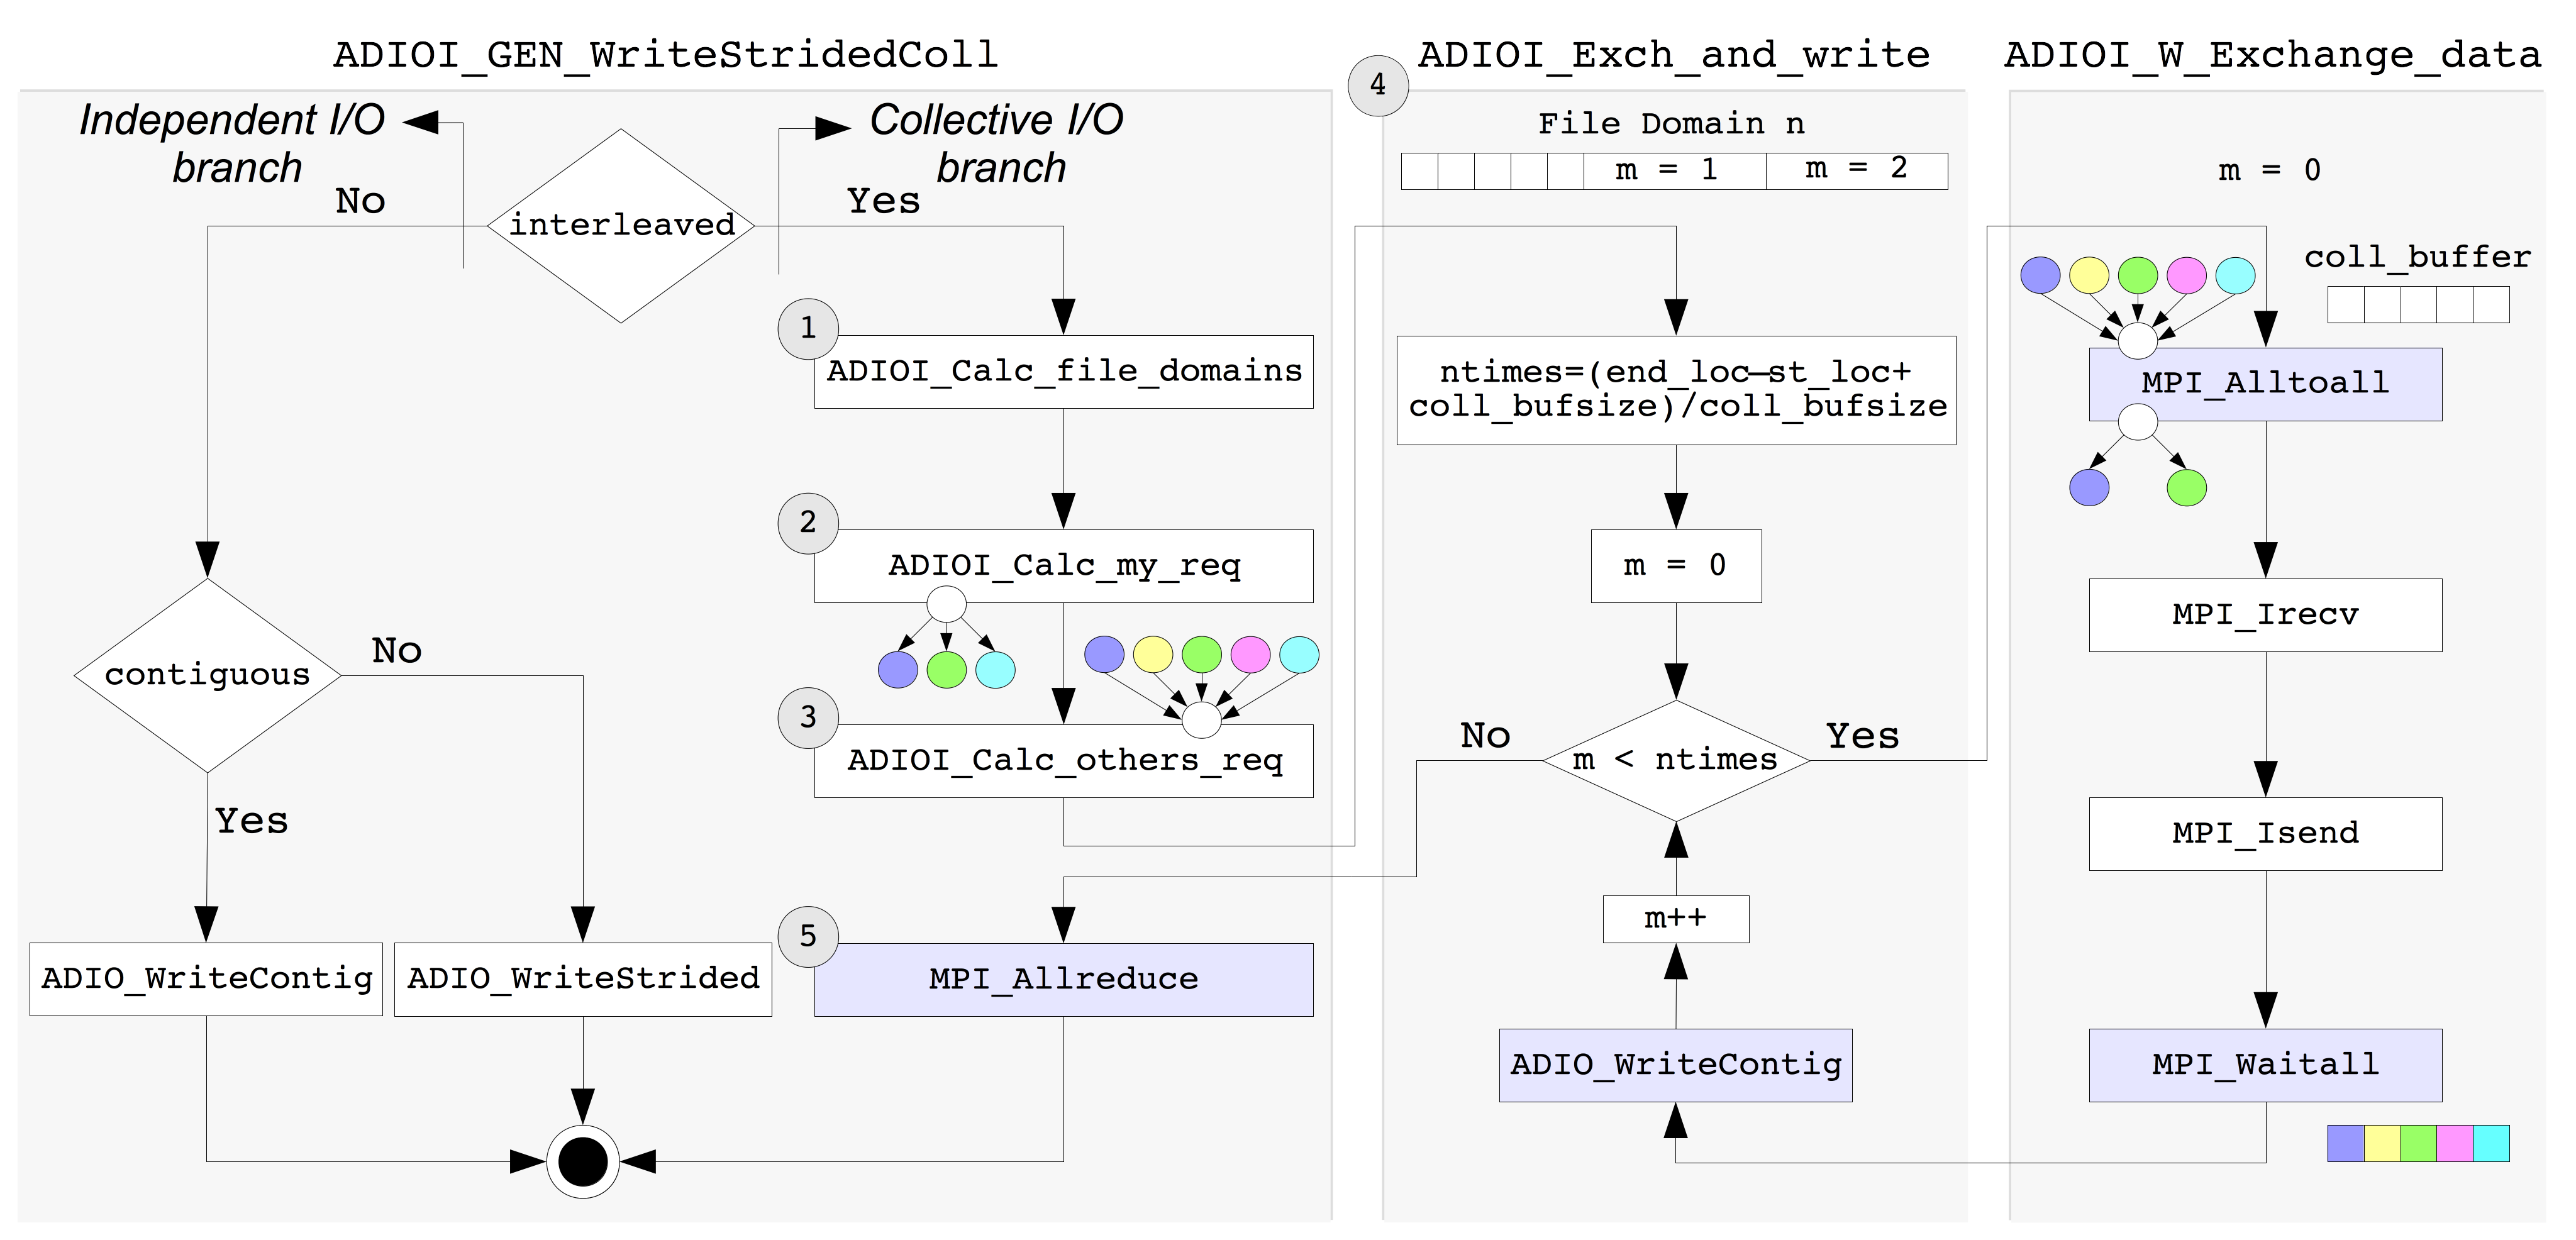
\includegraphics[width=\textwidth]{chapters/chapter3/figures/ext2ph}
  \caption{Collective I/O flow diagram for the write path in aggregators (non-aggregators neither receive nor write any data, just send it to aggregators). \codeword{MPI\_File\_write\_all()} invokes \codeword{ADIOI\_GEN\_WriteStridedColl()}. \codeword{ADIO\_WriteContig} is a macro that is replaced by \codeword{ADIOI\_GEN\_WriteContig()}. Performance critical functions for the collective I/O branch are highlighted in grey.}
  \label{figure: coll_io_impl}
\end{figure}

\begin{enumerate}
\item All processes taking part in the I/O operation exchange access pattern information with each other. The access pattern information is represented by start and end offsets for the accessed region (disregarding holes that may be present). Once file offsets are available, every process works out how big the global accessed region in the file is by taking maximum and minimum among all. The resulting byte range is divided by the number of available aggregators to build the so called `file domains' (contiguous byte ranges accessed independently by every aggregator).
\item Every process works out which file domains (and thus aggregators) its local data belongs to. In doing so, every process knows which aggregators it has to send (receive) data to (from), if any.
\item Every aggregator works out which other processes' requests map to its file domain. Doing so every aggregator knows what processes need to receive (in case of reads) or send (in case of writes) data for that particular file domain.
\item Actual two phase I/O starts. In the case of writes, that we exclusively consider here (the read case is similar), every process sends its data to the right aggregators (data shuffle phase) while these write the data to the parallel file system (data I/O phase). Data is written in blocks of predefined size (collective buffer size). If the size of the collective buffer is smaller than the file domain, the file domain is broken down into multiple sub-domains which are written in different rounds of the ext2ph algorithm. In order to handle multiple rounds of data shuffle and I/O, additional access information is required. This is disseminated by every process (collectively) to aggregators at the beginning of the data shuffle phase.
\item Once all the data has been written, all the processes must synchronise and exchange error codes. This is necessary to guarantee that it is safe to free the memory buffers containing the data.
\end{enumerate}

Figure~\ref{figure: coll_io_impl} shows how the previous steps map to the collective I/O implementation for the write operation. The collective write function (\codeword{MPI\_File\_write\_all()}) in ADIO is implemented through \codeword{ADIOI\_GEN\_WriteStridedColl()}. This is responsible for selecting the most suitable I/O method between those available. For example, independent I/O is selected if the access requests are not interleaved. Nevertheless, users can always enforce collective I/O by setting the appropriate MPI-IO hint. The \codeword{ADIOI\_Exch\_and\_write()} function contains the ext2ph algorithm implementation, including data shuffle and write methods. At the beginning of the data shuffle (\codeword{ADIOI\_W\_Exchange\_data()}) we have the dissemination function (\codeword{MPI\_Alltoall()}) used to exchange information concerning which part of the data has to be sent during a particular round of two phase I/O. 

There are three main contributors to collective I/O performance: (\textbf{a}) global synchronisation cost; (\textbf{b}) communication cost; and (\textbf{c}) write cost. \codeword{MPI\_Allreduce()} and \codeword{MPI\_Alltoall()} account for the global synchronisation cost. When a process reaches them it has to wait for all the other processes to arrive before continuing. \codeword{MPI\_Waitall()} accounts for communication cost since every process first issues all the non-blocking receives (if any) and sends, and afterwards waits for them to complete (refer to the right part of the diagram in Figure~\ref{figure: coll_io_impl}). Finally, \codeword{ADIO\_WriteContig()} accounts for write cost.

\subsubsection{Collective I/O Hints}
\label{subsec: hints}
As already said, collective I/O behaviour can be controlled by users through a dedicated set of MPI-IO hints. Users can control whether collective I/O should be enabled or disabled with \codeword{romio\_cb\_write} and \codeword{romio\_cb\_read}, for write and read operations respectively, how many aggregators should be used during a collective I/O operation with \codeword{cb\_nodes} and how big the collective buffer should be with \codeword{cb\_buffer\_size}. Table~\ref{table: coll_io_hints_table} summarises the hints just described (these are also reported in Table~\ref{table: romio-hints} along with all the other hints).

\begin{table}[!htb]
\centering
\ra{1.5}
\caption{Collective I/O hints in ROMIO.}
\newcolumntype{K}{>{\centering\arraybackslash} m{3cm}}
\newcolumntype{V}{>{\centering\arraybackslash} m{5.5cm}}
\begin{tabular}{KV}
\toprule
\bf \small Hint & \bf \small Description \\
\midrule
\small \codeword{romio\_cb\_write} & \small \codeword{enable} or \codeword{disable} collective writes \\
\small \codeword{romio\_cb\_read} & \small \codeword{enable} or \codeword{disable} collective reads \\
\small \codeword{cb\_buffer\_size} & \small set the collective buffer size [bytes]\\
\small \codeword{cb\_nodes} & \small set the number of aggregator processes\\
\bottomrule
\end{tabular}
\label{table: coll_io_hints_table}
\end{table}

Each of these hints has an effect on collective I/O performance. For example, by increasing the number of aggregators there will be a higher number of nodes writing to the parallel file system and thus a higher chance that one of these will experience variable performance due to load imbalance among available I/O servers, with increasing write time variation and associated global synchronisation cost. Furthermore, by increasing the collective buffer size users can reduce the number of two phase I/O rounds and, consequently, the number of global synchronisation events. Bigger collective buffers will also affect the write cost since more I/O servers will be accessed in parallel potentially increasing the aggregated I/O bandwidth.

Besides the hints described in Table~\ref{table: coll_io_hints_table}, there are other hints that do not directly concern collective I/O but affects its performance. The first is the \codeword{striping\_factor} hint, which defines how many I/O targets will be used to store the file. The second is the \codeword{striping\_unit} hint, which defines how big the data chunks written to each I/O target will be (in bytes). These two hints change the file characteristics in the parallel file system and typically the striping unit also defines the locking granularity for the file in the file system (e.g. Lustre).

%!TEX root = ../../main.tex
\section{The POSIX Advice API}
\label{sec: posix_advice_api}
The Linux kernel allows users to control page cache functionalities through the \texttt{posix\_fadvise()} system call: $$\textit{\textbf{int} posix\_fadvise(\textbf{int} fd, \textbf{off\_t} offset, \textbf{off\_t} len, \textbf{int} advice)}$$ This system call takes four input parameters: a valid file descriptor representing an open file, starting offset and length of the file region the advice will apply to, and finally the type of advice. The implementation provides five different types of advice, that reflect different aspects of caching. 

\begin{table}[!htb]
\centering
\ra{1.5}
\caption{Values for \textit{advice} in the \textit{posix\_fadvise()} system call}
\newcolumntype{K}{>{\centering\arraybackslash} m{4cm}}
\newcolumntype{V}{>{\centering\arraybackslash} m{5cm}}
\begin{tabular}{KV}
\toprule
\bf \small Advice & \bf \small Description \\
\midrule
\small \ttfamily POSIX\_FADV\_SEQUENTIAL & \small file I/O pattern is sequential \\
\small \ttfamily POSIX\_FADV\_RANDOM & \small file I/O pattern is random \\
\small \ttfamily POSIX\_FADV\_NORMAL & \small reset file I/O pattern to normal \\
\small \ttfamily POSIX\_FADV\_WILLNEED & \small file range will be needed \\
\small \ttfamily POSIX\_FADV\_DONTNEED & \small file range won't be needed \\
\small \ttfamily POSIX\_FADV\_NOREUSE & \small file is read once (not implemented) \\
\bottomrule
\end{tabular}
\label{table: advice_table}
\end{table}

The first two advice in Table~\ref{table: advice_table} have an impact on spatial locality of elements of the cache. \texttt{POSIX\_FADV\_SEQUENTIAL} can be used to advise the kernel that a file will be accessed sequentially. As result the kernel will double the maximum read-ahead window size in order to have a greedier read-ahead algorithm. \texttt{POSIX\_FADV\_RANDOM}, on the other hand, can be used when a file is accessed randomly and has the effect of completely disabling read-ahead, therefore only ever reading the requested data. Finally, \texttt{POSIX\_FADV\_NORMAL} can be used to cancel the previous two advice-messages and reset the read-ahead algorithm to its defaults. These three advice types apply to the whole file, the offset and length parameters are ignored for these `modes'.

Two of the remaining three advice types have an impact on the temporal locality of cache elements. \texttt{POSIX\_FADV\_WILLNEED} can be used to advise the kernel that the defined file region will be accessed soon, and therefore the kernel should prefetch the data and make it available in the page cache. \texttt{POSIX\_FADV\_DONTNEED} has the opposite effect, making the kernel release the specified file region from the cache, on the condition that the corresponding pages are clean (dirty pages are not released). Finally, the implementation for \texttt{POSIX\_FADV\_NOREUSE} is not provided in the kernel. %Table~\ref{table: advice_table} summarizes all the advice types just described.

One important aspect of \texttt{posix\_fadvise()} is that it is a synchronous system call. This means that every time an application invokes it, it blocks and returns only after the triggered read-ahead operations have completed. This represents a big limitation especially if we consider \texttt{POSIX\_FADV\_WILLNEED} that may need to prefetch an arbitrarily large chunk of data. In this scenario the application may be idle for a long period of time while the data is being retrieved by the file system.

%!TEX root = ../../main.tex
\section{The GPFS Hints API}
\label{sec: gpfs_hints_api}
Similarly to POSIX advice, GPFS provides users with the ability to control page pool functions through the \texttt{gpfs\_fcntl()} subroutine: $$\textit{\textbf{int} gpfs\_fcntl(\textbf{int} fileDesc, \textbf{void}* fcntlArgP)}$$ The subroutine takes two inputs: the file descriptor of the open file that hints will be applied to, and a pointer to a data structure residing in the application's address space. The indicated data structure contains all the information regarding what hints should be sent to GPFS. Specific hints are described by means of additional data structures that are contained in the main struct. Table~\ref{table: hints_table} summarizes all the available hints data structures and reports the corresponding description for each of them.

\begin{table}[!htb]
\centering
\ra{1.5}
\caption{GPFS hint data structures}
\newcolumntype{K}{>{\centering\arraybackslash} m{4.2cm}}
\newcolumntype{V}{>{\centering\arraybackslash} m{6cm}}
\begin{tabular}{KV}
\toprule
\bf \small Hint data structure & \bf \small Description \\
\midrule
\small \ttfamily gpfsAccessRange\_t & \small defines a file range to be accessed \\
\small \ttfamily gpfsFreeRange\_t & \small defines a file range to be released \\
\small \ttfamily gpfsMultipleAccessRange\_t & \small defines multiple file ranges to be accessed \\
\small \ttfamily gpfsClearFileCache\_t & \small releases all the page pool buffers for a certain file \\
\bottomrule
\end{tabular}
\label{table: hints_table}
\end{table}

Hints are not mandatory and GPFS can decide to accept or ignore them depending on specific conditions. Let us consider the multiple access range hint as an example (\texttt{gpfsMultipleAccessRange\_t} in table~\ref{table: hints_table}). The data structure corresponding to this hint is reported in Listing~\ref{list: mar}. 

\begin{lstlisting}[language=C, caption=Multiple Access Range Hint Data Structure, label={list: mar}]
#define GPFS_MAX_RANGE_COUNT 8

typedef struct
{
    int structLen;
    int structType;
    int accRangeCnt;
    int relRangeCnt;
    gpfsRangeArray_t accRangeArray[GPFS_MAX_RANGE_COUNT];
    gpfsRangeArray_t relRangeArray[GPFS_MAX_RANGE_COUNT];

} gpfsMultipleAccessRange_t;
\end{lstlisting}

\texttt{gpfsMultipleAccessRange\_t} contains two range arrays instead of just one: \texttt{accRangeArray}, used to define \texttt{accRangeCnt} blocks of the file that GPFS has to prefetch, and \texttt{relRangeArray} used to define \texttt{relRangeCnt} blocks of the file previously requested using \texttt{accRangeArray} and that are no longer needed. Unlike posix\_fadvise the user has to manage the list of blocks for which hints have been sent, updating whether they are still needed. Indeed, if the accessed blocks are not released, GPFS will stop accepting new hints once the maximum internal number of prefetch requests has been reached. 

\begin{lstlisting}[language=C, caption=Multiple Access Range Hint Initialisation and Submission, label={list: mar_example}]
void mercury::BlockCache::gpfsAccessReleaseBlock(
    std::vector<mercury::block_t>& access, 
    std::vector<mercury::block_t>& release)
{
  struct
  {
    gpfsFcntlHeader_t hdr;
    gpfsMultipleAccessRange_t marh;
  } accHint;

  accHint.hdr.totalLength = sizeof(accHint);
  accHint.hdr.fcntlVersion = GPFS_FCNTL_CURRENT_VERSION;
  accHint.hdr.fcntlReserved = 0;
  accHint.marh.structLen = sizeof(accHint.marh);
  accHint.marh.structType = GPFS_MULTIPLE_ACCESS_RANGE;
  accHint.marh.accRangeCnt = access.size();
  accHint.marh.relRangeCnt = release.size();

  for (i = 0; i < accHint.marh.accRangeCnt && 
      i < GPFS_MAX_RANGE_COUNT; i++)
  {
    accHint.marh.accRangeArray[i].blockNumber = 
      access[i].blockNumber_;
    accHint.marh.accRangeArray[i].start = 
      access[i].startOffset_;
    accHint.marh.accRangeArray[i].length = 
      access[i].blkLen_;
    accHint.marh.accRangeArray[i].isWrite = 
      access[i].isWrite_;
  }
  for (i = 0; i < accHint.marh.relRangeCnt && 
      i < GPFS_MAX_RANGE_COUNT; i++)
  {
    accHint.marh.relRangeArray[i].blockNumber = 
      release[i].blockNumber_;
    accHint.marh.relRangeArray[i].start = 
      release[i].startOffset_;
    accHint.marh.relRangeArray[i].length = 
      release[i].blkLen_;
    accHint.marh.relRangeArray[i].isWrite = 
      release[i].isWrite_;
  }

  /* issue the hints to gpfs */
  if (gpfs_fcntl(fd_, &accHint))
  {
    std::cerr << "gpfs_fcntl access hint failed for " <<
      fd_ << " errno=" << errno << " errorOffset=" <<
      accHint.hdr.errorOffset << std::endl;
    exit(EXIT_FAILURE);
  }

  /* remove the accessed and released blocks */
  access.erase(access.begin(), 
    access.begin() + accHint.marh.accRangeCnt);
  release.erase(release.begin(), 
    release.begin() + accHint.marh.relRangeCnt);
}
\end{lstlisting}

Listing~\ref{list: mar_example} shows an example for the multiple access range hint initialisation and submission. In the example the \codeword{gpfsAccessReleaseBlock()} function receives two vectors, each containing a number of regions that have to be prefetched (\texttt{access}) and released (\texttt{release}). Every access and release region defines the block number the current request starts from (\texttt{blockNumber\_}), the start offset inside the block (\texttt{startOffset\_}), the length of the block (\texttt{blkLen\_}) and if the request is a read or a write (\texttt{isWrite\_}). For every requested range the implementation fills the \codeword{accRangeArray} and the \codeword{relRangeArray} and finally submits the data structure to \codeword{gpfs\_fcntl()} to be served.


\chapter{Background on Guided I/O Intefaces}
In this chapter we present the state of the art in guided I/O interfaces for different software components of the I/O stack. Hints targeting different I/O parameters and mechanisms are presented and described in detail. Some of the presented hints will be useful to understand the design choices explored in the next chapters.

%!TEX source = ../../main.tex
\section{The MPI-IO Hints API}
\label{mpi-io-hints}
The MPI-IO standard allows users, as well as other libraries (e.g. HDF5, pnetCDF, etc), to control the internal behavior of the MPI-IO implementation (e.g. ROMIO) through a dedicated hints API. Hints are packed into a special object of type \codeword{MPI\_Info} and passed to the \codeword{MPI\_File\_open()} function. The open function transmits the hints to the underlying software modules that interpret them and take appropriate actions. An example of collective write and read hint initialisation and submission for the ROMIO middleware is shown in Listing~\ref{list: mpi-io-hint-example}.

\begin{lstlisting}[language=C, caption=MPI-IO Hints Initialisation and Submission, label={list: mpi-io-hint-example}]
  /* info object declaration */
  MPI_Info info;

  /* info object creation */
  MPI_Info_create(&info);

  /* info object initialisation */
  MPI_Info_set(info, "romio_cb_write", "enable");
  MPI_Info_set(info, "romio_cb_read", "enable");

  /* file object declaration */
  MPI_File file;

  /* file object initialisation */
  MPI_File_open(MPI_COMM_WORLD, "test_file", MPI_MODE_RDWR, 
    info, &file);

  /* perform I/O */

  /* file object finalisation */
  MPI_File_close(&file);

  /* info object destruction */
  MPI_Info_destroy(&info);
\end{lstlisting}

ROMIO exploits the MPI-IO hints API and defines its own set of hints to control the internal I/O transport behaviour. ROMIO hints are summarised in Table~\ref{table: romio-hints}. 

\begin{table}[!htb]
\centering
\ra{1.5}
\caption{ROMIO Hints and Corresponding Description}
\newcolumntype{K}{>{\centering\arraybackslash} m{4cm}}
\newcolumntype{V}{>{\centering\arraybackslash} m{5cm}}
\begin{tabular}{KV}
\toprule
\bf \small Hint & \bf \small Description \\
\midrule
\small \ttfamily  ind\_rd\_buffer\_size & \small independent read buffer size \\
\small \ttfamily  ind\_wr\_buffer\_size & \small independent write buffer size \\
\small \ttfamily  romio\_ds\_read & \small enable data sieving for reads \\
\small \ttfamily  romio\_ds\_write & \small enable data sieving for writes \\
\small \ttfamily  cb\_buffer\_size & \small collective buffer size \\
\small \ttfamily  cb\_nodes & \small number of aggregators in collective I/O \\
\small \ttfamily  romio\_cb\_read & \small enable collective I/O for reads \\
\small \ttfamily  romio\_cb\_write & \small enable collective I/O for writes \\
\small \ttfamily  romio\_no\_indep\_rw & \small enable deferred open (only aggregators open the file) \\
\small \ttfamily  cb\_config\_list & \small list of nodes to be selected as aggregators \\
\small \ttfamily  striping\_factor & \small number of I/O targets used to store the file \\
\small \ttfamily  striping\_unit & \small size of the stripe unit used to store the file \\
\small \ttfamily  start\_iodevice & \small I/O target storing the first stripe \\
\bottomrule
\end{tabular}
\label{table: romio-hints}
\end{table}

Hints are used to control the size of the I/O buffer both in independent and collective operations (i.e. \texttt{ind\_rd\_buffer\_size}, \texttt{ind\_wr\_buffer\_size} and \texttt{cb\_buffer\_size}), to enable I/O aggregation during reads and writes (i.e. \texttt{romio\_cb\_read} and \texttt{romio\_cb\_write}), and even to control file system specific parameters such as the number of I/O targets used to store the file (\texttt{striping\_factor}) or the size of the data blocks stored by every target (\texttt{striping\_unit}). Besides the ones reported in Table~\ref{table: romio-hints} there are additional file system specific hints (e.g. Lustre, PVFS, etc) that target the corresponding ROMIO file system drivers. For simplicity these are not reported in the table above. 

Hints are not MPI-IO specific, every middleware can exploit the MPI-IO hints API to support its own hints. In Chapter~\ref{chapter: deeper} we will discuss how to extend the ROMIO hints to support local storage file caching. Since we focus on improving the collective I/O implementation in ROMIO by introducing an additional memory tier, the next section is dedicated to collective I/O hints and implementation.

\subsection{Collective I/O in ROMIO}
\label{subsec: collio}
As already mentioned in the introduction, ROMIO is a popular implementation of the MPI-IO specification developed at the Argonne National Laboratory and currently supported by MPICH as well as OpenMPI and other packages. ROMIO provides parallel I/O functionalities for different file systems through the Abstract Device I/O interface (ADIO). Latest versions of ROMIO include support for Lustre, GPFS, PVFS and others through a dedicated ADIO driver. In ROMIO collective I/O is a parallel I/O technique designed to deliver high performance data access to distributed scientific applications that need to write data to a shared file efficiently.

\subsubsection{Two Phase I/O}
\label{subsubsec: ext2ph}
The core component of collective I/O is the `two phase I/O', also known as `extended two phase algorithm' (ext2ph)~\cite{ThakurC96}. The ROMIO implementation for collective I/O consists of several steps as following described:

\begin{figure}[!htb]
  \centering
  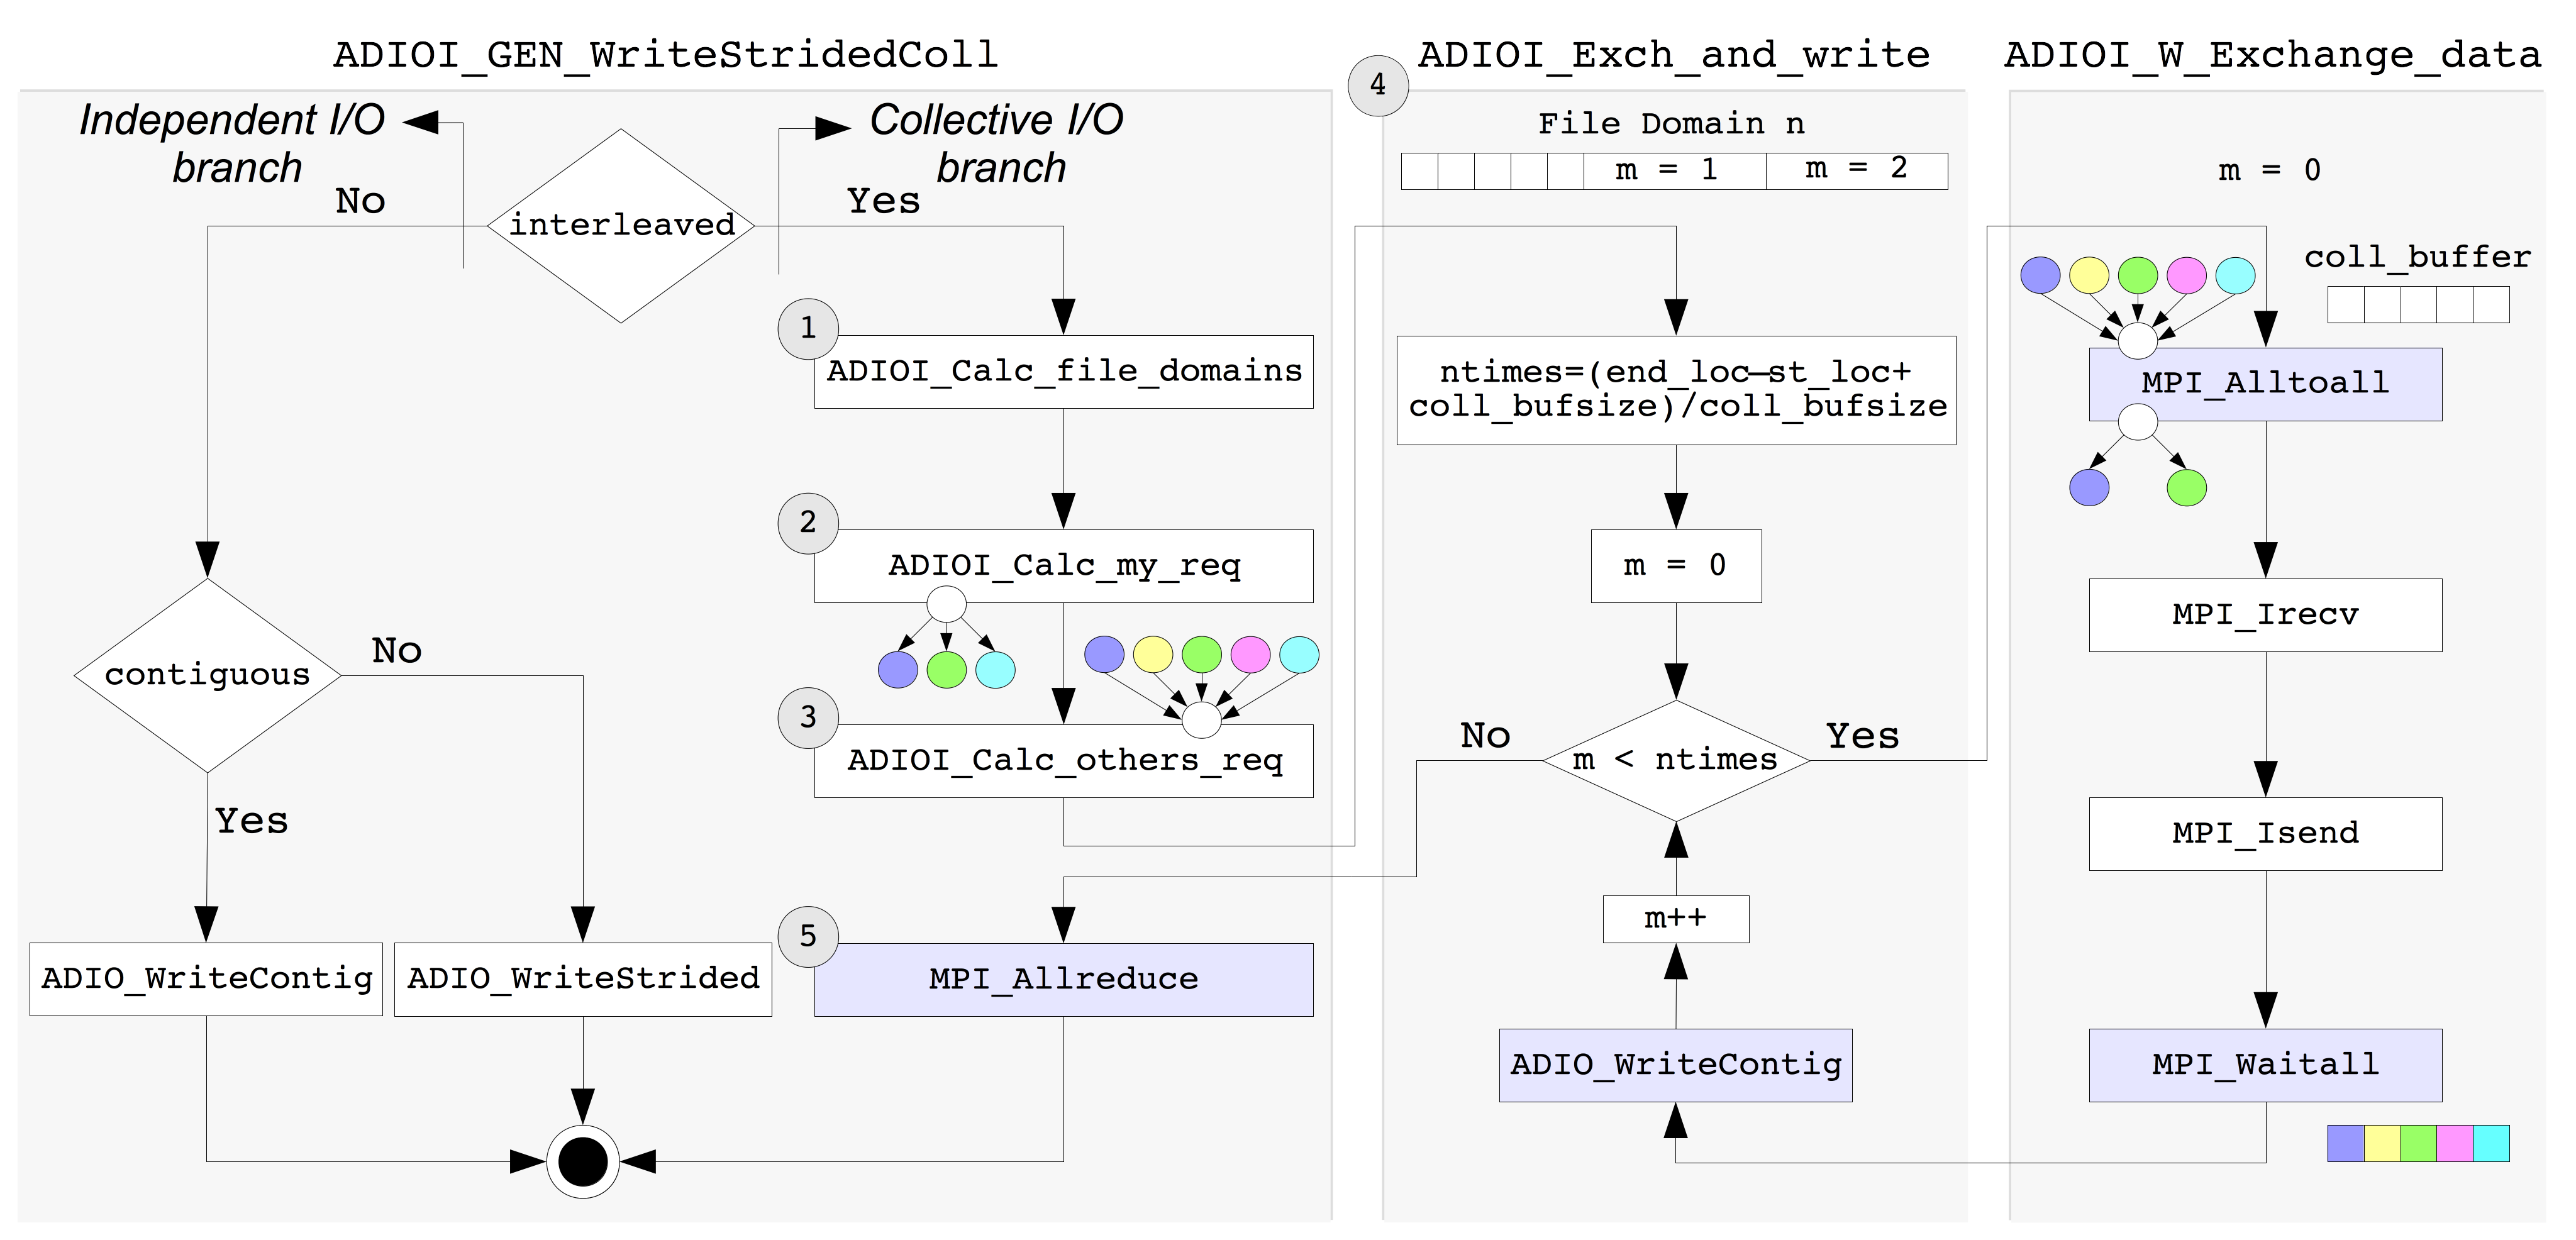
\includegraphics[width=\textwidth]{chapters/chapter3/figures/ext2ph}
  \caption{Collective I/O flow diagram for the write path in aggregators (non-aggregators neither receive nor write any data, just send it to aggregators). \codeword{MPI\_File\_write\_all()} invokes \codeword{ADIOI\_GEN\_WriteStridedColl()}. \codeword{ADIO\_WriteContig} is a macro that is replaced by \codeword{ADIOI\_GEN\_WriteContig()}. Performance critical functions for the collective I/O branch are highlighted in grey.}
  \label{figure: coll_io_impl}
\end{figure}

\begin{enumerate}
\item All processes taking part in the I/O operation exchange access pattern information with each other. The access pattern information is represented by start and end offsets for the accessed region (disregarding holes that may be present). Once file offsets are available, every process works out how big the global accessed region in the file is by taking maximum and minimum among all. The resulting byte range is divided by the number of available aggregators to build the so called `file domains' (contiguous byte ranges accessed independently by every aggregator).
\item Every process works out which file domains (and thus aggregators) its local data belongs to. In doing so, every process knows which aggregators it has to send (receive) data to (from), if any.
\item Every aggregator works out which other processes' requests map to its file domain. Doing so every aggregator knows what processes need to receive (in case of reads) or send (in case of writes) data for that particular file domain.
\item Actual two phase I/O starts. In the case of writes, that we exclusively consider here (the read case is similar), every process sends its data to the right aggregators (data shuffle phase) while these write the data to the parallel file system (data I/O phase). Data is written in blocks of predefined size (collective buffer size). If the size of the collective buffer is smaller than the file domain, the file domain is broken down into multiple sub-domains which are written in different rounds of the ext2ph algorithm. In order to handle multiple rounds of data shuffle and I/O, additional access information is required. This is disseminated by every process (collectively) to aggregators at the beginning of the data shuffle phase.
\item Once all the data has been written, all the processes must synchronise and exchange error codes. This is necessary to guarantee that it is safe to free the memory buffers containing the data.
\end{enumerate}

Figure~\ref{figure: coll_io_impl} shows how the previous steps map to the collective I/O implementation for the write operation. The collective write function (\codeword{MPI\_File\_write\_all()}) in ADIO is implemented through \codeword{ADIOI\_GEN\_WriteStridedColl()}. This is responsible for selecting the most suitable I/O method between those available. For example, independent I/O is selected if the access requests are not interleaved. Nevertheless, users can always enforce collective I/O by setting the appropriate MPI-IO hint. The \codeword{ADIOI\_Exch\_and\_write()} function contains the ext2ph algorithm implementation, including data shuffle and write methods. At the beginning of the data shuffle (\codeword{ADIOI\_W\_Exchange\_data()}) we have the dissemination function (\codeword{MPI\_Alltoall()}) used to exchange information concerning which part of the data has to be sent during a particular round of two phase I/O. 

There are three main contributors to collective I/O performance: (\textbf{a}) global synchronisation cost; (\textbf{b}) communication cost; and (\textbf{c}) write cost. \codeword{MPI\_Allreduce()} and \codeword{MPI\_Alltoall()} account for the global synchronisation cost. When a process reaches them it has to wait for all the other processes to arrive before continuing. \codeword{MPI\_Waitall()} accounts for communication cost since every process first issues all the non-blocking receives (if any) and sends, and afterwards waits for them to complete (refer to the right part of the diagram in Figure~\ref{figure: coll_io_impl}). Finally, \codeword{ADIO\_WriteContig()} accounts for write cost.

\subsubsection{Collective I/O Hints}
\label{subsec: hints}
As already said, collective I/O behaviour can be controlled by users through a dedicated set of MPI-IO hints. Users can control whether collective I/O should be enabled or disabled with \codeword{romio\_cb\_write} and \codeword{romio\_cb\_read}, for write and read operations respectively, how many aggregators should be used during a collective I/O operation with \codeword{cb\_nodes} and how big the collective buffer should be with \codeword{cb\_buffer\_size}. Table~\ref{table: coll_io_hints_table} summarises the hints just described (these are also reported in Table~\ref{table: romio-hints} along with all the other hints).

\begin{table}[!htb]
\centering
\ra{1.5}
\caption{Collective I/O hints in ROMIO.}
\newcolumntype{K}{>{\centering\arraybackslash} m{3cm}}
\newcolumntype{V}{>{\centering\arraybackslash} m{5.5cm}}
\begin{tabular}{KV}
\toprule
\bf \small Hint & \bf \small Description \\
\midrule
\small \codeword{romio\_cb\_write} & \small \codeword{enable} or \codeword{disable} collective writes \\
\small \codeword{romio\_cb\_read} & \small \codeword{enable} or \codeword{disable} collective reads \\
\small \codeword{cb\_buffer\_size} & \small set the collective buffer size [bytes]\\
\small \codeword{cb\_nodes} & \small set the number of aggregator processes\\
\bottomrule
\end{tabular}
\label{table: coll_io_hints_table}
\end{table}

Each of these hints has an effect on collective I/O performance. For example, by increasing the number of aggregators there will be a higher number of nodes writing to the parallel file system and thus a higher chance that one of these will experience variable performance due to load imbalance among available I/O servers, with increasing write time variation and associated global synchronisation cost. Furthermore, by increasing the collective buffer size users can reduce the number of two phase I/O rounds and, consequently, the number of global synchronisation events. Bigger collective buffers will also affect the write cost since more I/O servers will be accessed in parallel potentially increasing the aggregated I/O bandwidth.

Besides the hints described in Table~\ref{table: coll_io_hints_table}, there are other hints that do not directly concern collective I/O but affects its performance. The first is the \codeword{striping\_factor} hint, which defines how many I/O targets will be used to store the file. The second is the \codeword{striping\_unit} hint, which defines how big the data chunks written to each I/O target will be (in bytes). These two hints change the file characteristics in the parallel file system and typically the striping unit also defines the locking granularity for the file in the file system (e.g. Lustre).

%!TEX root = ../../main.tex
\section{The POSIX Advice API}
\label{sec: posix_advice_api}
The Linux kernel allows users to control page cache functionalities through the \texttt{posix\_fadvise()} system call: $$\textit{\textbf{int} posix\_fadvise(\textbf{int} fd, \textbf{off\_t} offset, \textbf{off\_t} len, \textbf{int} advice)}$$ This system call takes four input parameters: a valid file descriptor representing an open file, starting offset and length of the file region the advice will apply to, and finally the type of advice. The implementation provides five different types of advice, that reflect different aspects of caching. 

\begin{table}[!htb]
\centering
\ra{1.5}
\caption{Values for \textit{advice} in the \textit{posix\_fadvise()} system call}
\newcolumntype{K}{>{\centering\arraybackslash} m{4cm}}
\newcolumntype{V}{>{\centering\arraybackslash} m{5cm}}
\begin{tabular}{KV}
\toprule
\bf \small Advice & \bf \small Description \\
\midrule
\small \ttfamily POSIX\_FADV\_SEQUENTIAL & \small file I/O pattern is sequential \\
\small \ttfamily POSIX\_FADV\_RANDOM & \small file I/O pattern is random \\
\small \ttfamily POSIX\_FADV\_NORMAL & \small reset file I/O pattern to normal \\
\small \ttfamily POSIX\_FADV\_WILLNEED & \small file range will be needed \\
\small \ttfamily POSIX\_FADV\_DONTNEED & \small file range won't be needed \\
\small \ttfamily POSIX\_FADV\_NOREUSE & \small file is read once (not implemented) \\
\bottomrule
\end{tabular}
\label{table: advice_table}
\end{table}

The first two advice in Table~\ref{table: advice_table} have an impact on spatial locality of elements of the cache. \texttt{POSIX\_FADV\_SEQUENTIAL} can be used to advise the kernel that a file will be accessed sequentially. As result the kernel will double the maximum read-ahead window size in order to have a greedier read-ahead algorithm. \texttt{POSIX\_FADV\_RANDOM}, on the other hand, can be used when a file is accessed randomly and has the effect of completely disabling read-ahead, therefore only ever reading the requested data. Finally, \texttt{POSIX\_FADV\_NORMAL} can be used to cancel the previous two advice-messages and reset the read-ahead algorithm to its defaults. These three advice types apply to the whole file, the offset and length parameters are ignored for these `modes'.

Two of the remaining three advice types have an impact on the temporal locality of cache elements. \texttt{POSIX\_FADV\_WILLNEED} can be used to advise the kernel that the defined file region will be accessed soon, and therefore the kernel should prefetch the data and make it available in the page cache. \texttt{POSIX\_FADV\_DONTNEED} has the opposite effect, making the kernel release the specified file region from the cache, on the condition that the corresponding pages are clean (dirty pages are not released). Finally, the implementation for \texttt{POSIX\_FADV\_NOREUSE} is not provided in the kernel. %Table~\ref{table: advice_table} summarizes all the advice types just described.

One important aspect of \texttt{posix\_fadvise()} is that it is a synchronous system call. This means that every time an application invokes it, it blocks and returns only after the triggered read-ahead operations have completed. This represents a big limitation especially if we consider \texttt{POSIX\_FADV\_WILLNEED} that may need to prefetch an arbitrarily large chunk of data. In this scenario the application may be idle for a long period of time while the data is being retrieved by the file system.

%!TEX root = ../../main.tex
\section{The GPFS Hints API}
\label{sec: gpfs_hints_api}
Similarly to POSIX advice, GPFS provides users with the ability to control page pool functions through the \texttt{gpfs\_fcntl()} subroutine: $$\textit{\textbf{int} gpfs\_fcntl(\textbf{int} fileDesc, \textbf{void}* fcntlArgP)}$$ The subroutine takes two inputs: the file descriptor of the open file that hints will be applied to, and a pointer to a data structure residing in the application's address space. The indicated data structure contains all the information regarding what hints should be sent to GPFS. Specific hints are described by means of additional data structures that are contained in the main struct. Table~\ref{table: hints_table} summarizes all the available hints data structures and reports the corresponding description for each of them.

\begin{table}[!htb]
\centering
\ra{1.5}
\caption{GPFS hint data structures}
\newcolumntype{K}{>{\centering\arraybackslash} m{4.2cm}}
\newcolumntype{V}{>{\centering\arraybackslash} m{6cm}}
\begin{tabular}{KV}
\toprule
\bf \small Hint data structure & \bf \small Description \\
\midrule
\small \ttfamily gpfsAccessRange\_t & \small defines a file range to be accessed \\
\small \ttfamily gpfsFreeRange\_t & \small defines a file range to be released \\
\small \ttfamily gpfsMultipleAccessRange\_t & \small defines multiple file ranges to be accessed \\
\small \ttfamily gpfsClearFileCache\_t & \small releases all the page pool buffers for a certain file \\
\bottomrule
\end{tabular}
\label{table: hints_table}
\end{table}

Hints are not mandatory and GPFS can decide to accept or ignore them depending on specific conditions. Let us consider the multiple access range hint as an example (\texttt{gpfsMultipleAccessRange\_t} in table~\ref{table: hints_table}). The data structure corresponding to this hint is reported in Listing~\ref{list: mar}. 

\begin{lstlisting}[language=C, caption=Multiple Access Range Hint Data Structure, label={list: mar}]
#define GPFS_MAX_RANGE_COUNT 8

typedef struct
{
    int structLen;
    int structType;
    int accRangeCnt;
    int relRangeCnt;
    gpfsRangeArray_t accRangeArray[GPFS_MAX_RANGE_COUNT];
    gpfsRangeArray_t relRangeArray[GPFS_MAX_RANGE_COUNT];

} gpfsMultipleAccessRange_t;
\end{lstlisting}

\texttt{gpfsMultipleAccessRange\_t} contains two range arrays instead of just one: \texttt{accRangeArray}, used to define \texttt{accRangeCnt} blocks of the file that GPFS has to prefetch, and \texttt{relRangeArray} used to define \texttt{relRangeCnt} blocks of the file previously requested using \texttt{accRangeArray} and that are no longer needed. Unlike posix\_fadvise the user has to manage the list of blocks for which hints have been sent, updating whether they are still needed. Indeed, if the accessed blocks are not released, GPFS will stop accepting new hints once the maximum internal number of prefetch requests has been reached. 

\begin{lstlisting}[language=C, caption=Multiple Access Range Hint Initialisation and Submission, label={list: mar_example}]
void mercury::BlockCache::gpfsAccessReleaseBlock(
    std::vector<mercury::block_t>& access, 
    std::vector<mercury::block_t>& release)
{
  struct
  {
    gpfsFcntlHeader_t hdr;
    gpfsMultipleAccessRange_t marh;
  } accHint;

  accHint.hdr.totalLength = sizeof(accHint);
  accHint.hdr.fcntlVersion = GPFS_FCNTL_CURRENT_VERSION;
  accHint.hdr.fcntlReserved = 0;
  accHint.marh.structLen = sizeof(accHint.marh);
  accHint.marh.structType = GPFS_MULTIPLE_ACCESS_RANGE;
  accHint.marh.accRangeCnt = access.size();
  accHint.marh.relRangeCnt = release.size();

  for (i = 0; i < accHint.marh.accRangeCnt && 
      i < GPFS_MAX_RANGE_COUNT; i++)
  {
    accHint.marh.accRangeArray[i].blockNumber = 
      access[i].blockNumber_;
    accHint.marh.accRangeArray[i].start = 
      access[i].startOffset_;
    accHint.marh.accRangeArray[i].length = 
      access[i].blkLen_;
    accHint.marh.accRangeArray[i].isWrite = 
      access[i].isWrite_;
  }
  for (i = 0; i < accHint.marh.relRangeCnt && 
      i < GPFS_MAX_RANGE_COUNT; i++)
  {
    accHint.marh.relRangeArray[i].blockNumber = 
      release[i].blockNumber_;
    accHint.marh.relRangeArray[i].start = 
      release[i].startOffset_;
    accHint.marh.relRangeArray[i].length = 
      release[i].blkLen_;
    accHint.marh.relRangeArray[i].isWrite = 
      release[i].isWrite_;
  }

  /* issue the hints to gpfs */
  if (gpfs_fcntl(fd_, &accHint))
  {
    std::cerr << "gpfs_fcntl access hint failed for " <<
      fd_ << " errno=" << errno << " errorOffset=" <<
      accHint.hdr.errorOffset << std::endl;
    exit(EXIT_FAILURE);
  }

  /* remove the accessed and released blocks */
  access.erase(access.begin(), 
    access.begin() + accHint.marh.accRangeCnt);
  release.erase(release.begin(), 
    release.begin() + accHint.marh.relRangeCnt);
}
\end{lstlisting}

Listing~\ref{list: mar_example} shows an example for the multiple access range hint initialisation and submission. In the example the \codeword{gpfsAccessReleaseBlock()} function receives two vectors, each containing a number of regions that have to be prefetched (\texttt{access}) and released (\texttt{release}). Every access and release region defines the block number the current request starts from (\texttt{blockNumber\_}), the start offset inside the block (\texttt{startOffset\_}), the length of the block (\texttt{blkLen\_}) and if the request is a read or a write (\texttt{isWrite\_}). For every requested range the implementation fills the \codeword{accRangeArray} and the \codeword{relRangeArray} and finally submits the data structure to \codeword{gpfs\_fcntl()} to be served.


\chapter{Background on Guided I/O Intefaces}
In this chapter we present the state of the art in guided I/O interfaces for different software components of the I/O stack. Hints targeting different I/O parameters and mechanisms are presented and described in detail. Some of the presented hints will be useful to understand the design choices explored in the next chapters.

%!TEX source = ../../main.tex
\section{The MPI-IO Hints API}
\label{mpi-io-hints}
The MPI-IO standard allows users, as well as other libraries (e.g. HDF5, pnetCDF, etc), to control the internal behavior of the MPI-IO implementation (e.g. ROMIO) through a dedicated hints API. Hints are packed into a special object of type \codeword{MPI\_Info} and passed to the \codeword{MPI\_File\_open()} function. The open function transmits the hints to the underlying software modules that interpret them and take appropriate actions. An example of collective write and read hint initialisation and submission for the ROMIO middleware is shown in Listing~\ref{list: mpi-io-hint-example}.

\begin{lstlisting}[language=C, caption=MPI-IO Hints Initialisation and Submission, label={list: mpi-io-hint-example}]
  /* info object declaration */
  MPI_Info info;

  /* info object creation */
  MPI_Info_create(&info);

  /* info object initialisation */
  MPI_Info_set(info, "romio_cb_write", "enable");
  MPI_Info_set(info, "romio_cb_read", "enable");

  /* file object declaration */
  MPI_File file;

  /* file object initialisation */
  MPI_File_open(MPI_COMM_WORLD, "test_file", MPI_MODE_RDWR, 
    info, &file);

  /* perform I/O */

  /* file object finalisation */
  MPI_File_close(&file);

  /* info object destruction */
  MPI_Info_destroy(&info);
\end{lstlisting}

ROMIO exploits the MPI-IO hints API and defines its own set of hints to control the internal I/O transport behaviour. ROMIO hints are summarised in Table~\ref{table: romio-hints}. 

\begin{table}[!htb]
\centering
\ra{1.5}
\caption{ROMIO Hints and Corresponding Description}
\newcolumntype{K}{>{\centering\arraybackslash} m{4cm}}
\newcolumntype{V}{>{\centering\arraybackslash} m{5cm}}
\begin{tabular}{KV}
\toprule
\bf \small Hint & \bf \small Description \\
\midrule
\small \ttfamily  ind\_rd\_buffer\_size & \small independent read buffer size \\
\small \ttfamily  ind\_wr\_buffer\_size & \small independent write buffer size \\
\small \ttfamily  romio\_ds\_read & \small enable data sieving for reads \\
\small \ttfamily  romio\_ds\_write & \small enable data sieving for writes \\
\small \ttfamily  cb\_buffer\_size & \small collective buffer size \\
\small \ttfamily  cb\_nodes & \small number of aggregators in collective I/O \\
\small \ttfamily  romio\_cb\_read & \small enable collective I/O for reads \\
\small \ttfamily  romio\_cb\_write & \small enable collective I/O for writes \\
\small \ttfamily  romio\_no\_indep\_rw & \small enable deferred open (only aggregators open the file) \\
\small \ttfamily  cb\_config\_list & \small list of nodes to be selected as aggregators \\
\small \ttfamily  striping\_factor & \small number of I/O targets used to store the file \\
\small \ttfamily  striping\_unit & \small size of the stripe unit used to store the file \\
\small \ttfamily  start\_iodevice & \small I/O target storing the first stripe \\
\bottomrule
\end{tabular}
\label{table: romio-hints}
\end{table}

Hints are used to control the size of the I/O buffer both in independent and collective operations (i.e. \texttt{ind\_rd\_buffer\_size}, \texttt{ind\_wr\_buffer\_size} and \texttt{cb\_buffer\_size}), to enable I/O aggregation during reads and writes (i.e. \texttt{romio\_cb\_read} and \texttt{romio\_cb\_write}), and even to control file system specific parameters such as the number of I/O targets used to store the file (\texttt{striping\_factor}) or the size of the data blocks stored by every target (\texttt{striping\_unit}). Besides the ones reported in Table~\ref{table: romio-hints} there are additional file system specific hints (e.g. Lustre, PVFS, etc) that target the corresponding ROMIO file system drivers. For simplicity these are not reported in the table above. 

Hints are not MPI-IO specific, every middleware can exploit the MPI-IO hints API to support its own hints. In Chapter~\ref{chapter: deeper} we will discuss how to extend the ROMIO hints to support local storage file caching. Since we focus on improving the collective I/O implementation in ROMIO by introducing an additional memory tier, the next section is dedicated to collective I/O hints and implementation.

\subsection{Collective I/O in ROMIO}
\label{subsec: collio}
As already mentioned in the introduction, ROMIO is a popular implementation of the MPI-IO specification developed at the Argonne National Laboratory and currently supported by MPICH as well as OpenMPI and other packages. ROMIO provides parallel I/O functionalities for different file systems through the Abstract Device I/O interface (ADIO). Latest versions of ROMIO include support for Lustre, GPFS, PVFS and others through a dedicated ADIO driver. In ROMIO collective I/O is a parallel I/O technique designed to deliver high performance data access to distributed scientific applications that need to write data to a shared file efficiently.

\subsubsection{Two Phase I/O}
\label{subsubsec: ext2ph}
The core component of collective I/O is the `two phase I/O', also known as `extended two phase algorithm' (ext2ph)~\cite{ThakurC96}. The ROMIO implementation for collective I/O consists of several steps as following described:

\begin{figure}[!htb]
  \centering
  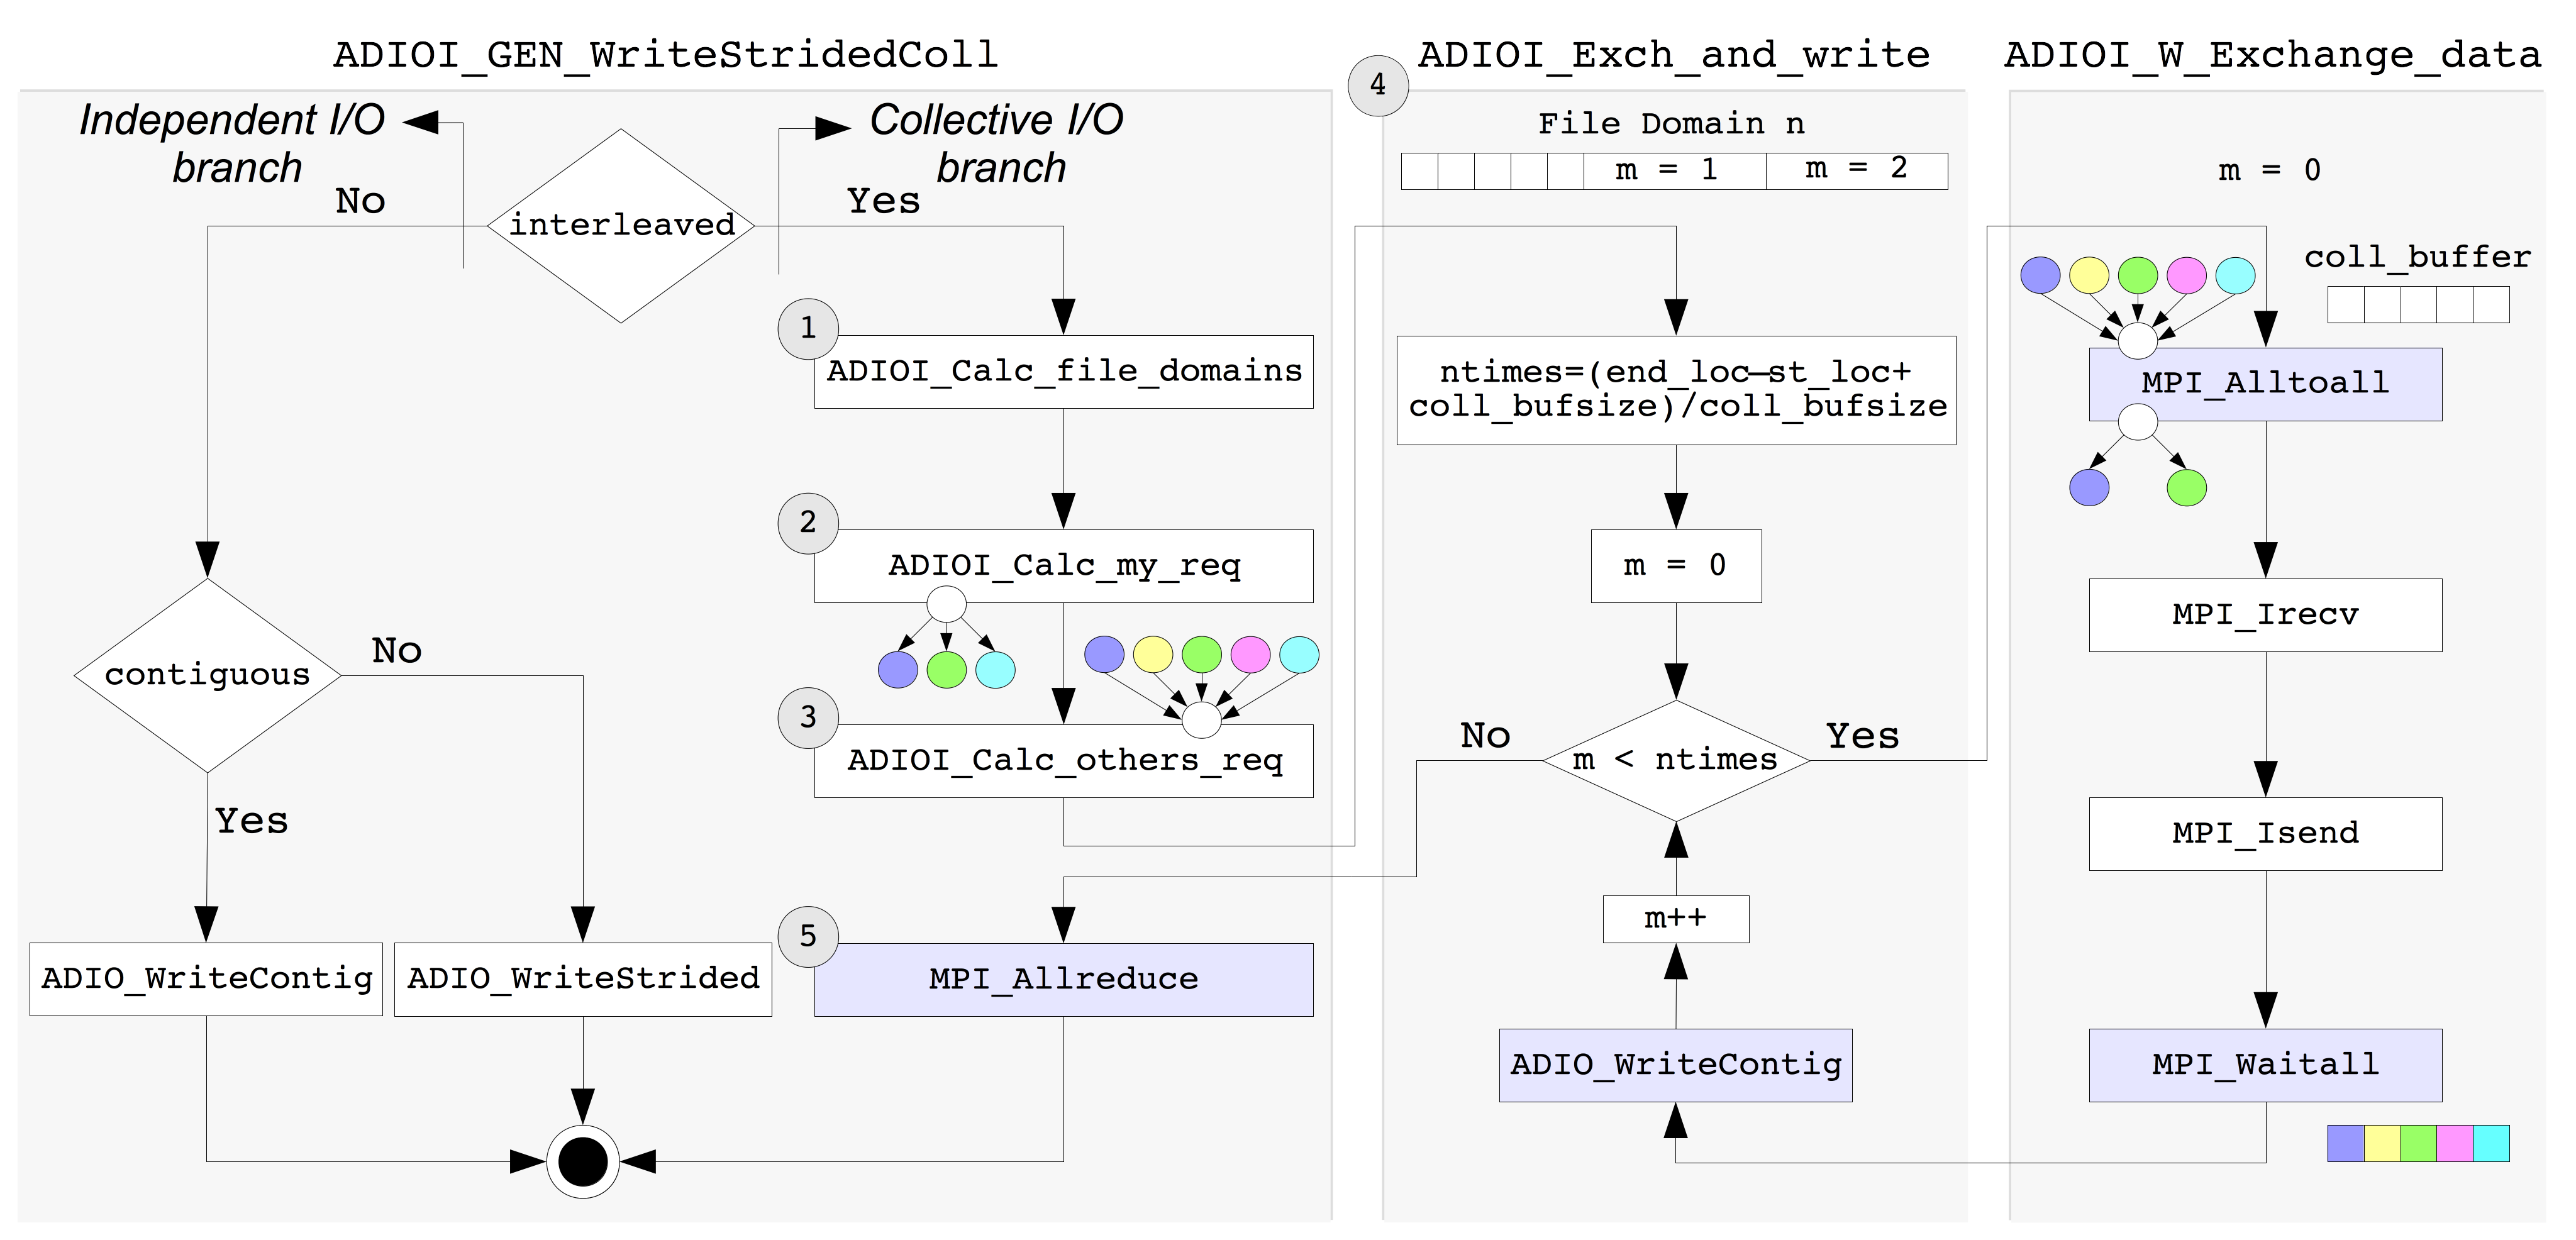
\includegraphics[width=\textwidth]{chapters/chapter3/figures/ext2ph}
  \caption{Collective I/O flow diagram for the write path in aggregators (non-aggregators neither receive nor write any data, just send it to aggregators). \codeword{MPI\_File\_write\_all()} invokes \codeword{ADIOI\_GEN\_WriteStridedColl()}. \codeword{ADIO\_WriteContig} is a macro that is replaced by \codeword{ADIOI\_GEN\_WriteContig()}. Performance critical functions for the collective I/O branch are highlighted in grey.}
  \label{figure: coll_io_impl}
\end{figure}

\begin{enumerate}
\item All processes taking part in the I/O operation exchange access pattern information with each other. The access pattern information is represented by start and end offsets for the accessed region (disregarding holes that may be present). Once file offsets are available, every process works out how big the global accessed region in the file is by taking maximum and minimum among all. The resulting byte range is divided by the number of available aggregators to build the so called `file domains' (contiguous byte ranges accessed independently by every aggregator).
\item Every process works out which file domains (and thus aggregators) its local data belongs to. In doing so, every process knows which aggregators it has to send (receive) data to (from), if any.
\item Every aggregator works out which other processes' requests map to its file domain. Doing so every aggregator knows what processes need to receive (in case of reads) or send (in case of writes) data for that particular file domain.
\item Actual two phase I/O starts. In the case of writes, that we exclusively consider here (the read case is similar), every process sends its data to the right aggregators (data shuffle phase) while these write the data to the parallel file system (data I/O phase). Data is written in blocks of predefined size (collective buffer size). If the size of the collective buffer is smaller than the file domain, the file domain is broken down into multiple sub-domains which are written in different rounds of the ext2ph algorithm. In order to handle multiple rounds of data shuffle and I/O, additional access information is required. This is disseminated by every process (collectively) to aggregators at the beginning of the data shuffle phase.
\item Once all the data has been written, all the processes must synchronise and exchange error codes. This is necessary to guarantee that it is safe to free the memory buffers containing the data.
\end{enumerate}

Figure~\ref{figure: coll_io_impl} shows how the previous steps map to the collective I/O implementation for the write operation. The collective write function (\codeword{MPI\_File\_write\_all()}) in ADIO is implemented through \codeword{ADIOI\_GEN\_WriteStridedColl()}. This is responsible for selecting the most suitable I/O method between those available. For example, independent I/O is selected if the access requests are not interleaved. Nevertheless, users can always enforce collective I/O by setting the appropriate MPI-IO hint. The \codeword{ADIOI\_Exch\_and\_write()} function contains the ext2ph algorithm implementation, including data shuffle and write methods. At the beginning of the data shuffle (\codeword{ADIOI\_W\_Exchange\_data()}) we have the dissemination function (\codeword{MPI\_Alltoall()}) used to exchange information concerning which part of the data has to be sent during a particular round of two phase I/O. 

There are three main contributors to collective I/O performance: (\textbf{a}) global synchronisation cost; (\textbf{b}) communication cost; and (\textbf{c}) write cost. \codeword{MPI\_Allreduce()} and \codeword{MPI\_Alltoall()} account for the global synchronisation cost. When a process reaches them it has to wait for all the other processes to arrive before continuing. \codeword{MPI\_Waitall()} accounts for communication cost since every process first issues all the non-blocking receives (if any) and sends, and afterwards waits for them to complete (refer to the right part of the diagram in Figure~\ref{figure: coll_io_impl}). Finally, \codeword{ADIO\_WriteContig()} accounts for write cost.

\subsubsection{Collective I/O Hints}
\label{subsec: hints}
As already said, collective I/O behaviour can be controlled by users through a dedicated set of MPI-IO hints. Users can control whether collective I/O should be enabled or disabled with \codeword{romio\_cb\_write} and \codeword{romio\_cb\_read}, for write and read operations respectively, how many aggregators should be used during a collective I/O operation with \codeword{cb\_nodes} and how big the collective buffer should be with \codeword{cb\_buffer\_size}. Table~\ref{table: coll_io_hints_table} summarises the hints just described (these are also reported in Table~\ref{table: romio-hints} along with all the other hints).

\begin{table}[!htb]
\centering
\ra{1.5}
\caption{Collective I/O hints in ROMIO.}
\newcolumntype{K}{>{\centering\arraybackslash} m{3cm}}
\newcolumntype{V}{>{\centering\arraybackslash} m{5.5cm}}
\begin{tabular}{KV}
\toprule
\bf \small Hint & \bf \small Description \\
\midrule
\small \codeword{romio\_cb\_write} & \small \codeword{enable} or \codeword{disable} collective writes \\
\small \codeword{romio\_cb\_read} & \small \codeword{enable} or \codeword{disable} collective reads \\
\small \codeword{cb\_buffer\_size} & \small set the collective buffer size [bytes]\\
\small \codeword{cb\_nodes} & \small set the number of aggregator processes\\
\bottomrule
\end{tabular}
\label{table: coll_io_hints_table}
\end{table}

Each of these hints has an effect on collective I/O performance. For example, by increasing the number of aggregators there will be a higher number of nodes writing to the parallel file system and thus a higher chance that one of these will experience variable performance due to load imbalance among available I/O servers, with increasing write time variation and associated global synchronisation cost. Furthermore, by increasing the collective buffer size users can reduce the number of two phase I/O rounds and, consequently, the number of global synchronisation events. Bigger collective buffers will also affect the write cost since more I/O servers will be accessed in parallel potentially increasing the aggregated I/O bandwidth.

Besides the hints described in Table~\ref{table: coll_io_hints_table}, there are other hints that do not directly concern collective I/O but affects its performance. The first is the \codeword{striping\_factor} hint, which defines how many I/O targets will be used to store the file. The second is the \codeword{striping\_unit} hint, which defines how big the data chunks written to each I/O target will be (in bytes). These two hints change the file characteristics in the parallel file system and typically the striping unit also defines the locking granularity for the file in the file system (e.g. Lustre).

%!TEX root = ../../main.tex
\section{The POSIX Advice API}
\label{sec: posix_advice_api}
The Linux kernel allows users to control page cache functionalities through the \texttt{posix\_fadvise()} system call: $$\textit{\textbf{int} posix\_fadvise(\textbf{int} fd, \textbf{off\_t} offset, \textbf{off\_t} len, \textbf{int} advice)}$$ This system call takes four input parameters: a valid file descriptor representing an open file, starting offset and length of the file region the advice will apply to, and finally the type of advice. The implementation provides five different types of advice, that reflect different aspects of caching. 

\begin{table}[!htb]
\centering
\ra{1.5}
\caption{Values for \textit{advice} in the \textit{posix\_fadvise()} system call}
\newcolumntype{K}{>{\centering\arraybackslash} m{4cm}}
\newcolumntype{V}{>{\centering\arraybackslash} m{5cm}}
\begin{tabular}{KV}
\toprule
\bf \small Advice & \bf \small Description \\
\midrule
\small \ttfamily POSIX\_FADV\_SEQUENTIAL & \small file I/O pattern is sequential \\
\small \ttfamily POSIX\_FADV\_RANDOM & \small file I/O pattern is random \\
\small \ttfamily POSIX\_FADV\_NORMAL & \small reset file I/O pattern to normal \\
\small \ttfamily POSIX\_FADV\_WILLNEED & \small file range will be needed \\
\small \ttfamily POSIX\_FADV\_DONTNEED & \small file range won't be needed \\
\small \ttfamily POSIX\_FADV\_NOREUSE & \small file is read once (not implemented) \\
\bottomrule
\end{tabular}
\label{table: advice_table}
\end{table}

The first two advice in Table~\ref{table: advice_table} have an impact on spatial locality of elements of the cache. \texttt{POSIX\_FADV\_SEQUENTIAL} can be used to advise the kernel that a file will be accessed sequentially. As result the kernel will double the maximum read-ahead window size in order to have a greedier read-ahead algorithm. \texttt{POSIX\_FADV\_RANDOM}, on the other hand, can be used when a file is accessed randomly and has the effect of completely disabling read-ahead, therefore only ever reading the requested data. Finally, \texttt{POSIX\_FADV\_NORMAL} can be used to cancel the previous two advice-messages and reset the read-ahead algorithm to its defaults. These three advice types apply to the whole file, the offset and length parameters are ignored for these `modes'.

Two of the remaining three advice types have an impact on the temporal locality of cache elements. \texttt{POSIX\_FADV\_WILLNEED} can be used to advise the kernel that the defined file region will be accessed soon, and therefore the kernel should prefetch the data and make it available in the page cache. \texttt{POSIX\_FADV\_DONTNEED} has the opposite effect, making the kernel release the specified file region from the cache, on the condition that the corresponding pages are clean (dirty pages are not released). Finally, the implementation for \texttt{POSIX\_FADV\_NOREUSE} is not provided in the kernel. %Table~\ref{table: advice_table} summarizes all the advice types just described.

One important aspect of \texttt{posix\_fadvise()} is that it is a synchronous system call. This means that every time an application invokes it, it blocks and returns only after the triggered read-ahead operations have completed. This represents a big limitation especially if we consider \texttt{POSIX\_FADV\_WILLNEED} that may need to prefetch an arbitrarily large chunk of data. In this scenario the application may be idle for a long period of time while the data is being retrieved by the file system.

%!TEX root = ../../main.tex
\section{The GPFS Hints API}
\label{sec: gpfs_hints_api}
Similarly to POSIX advice, GPFS provides users with the ability to control page pool functions through the \texttt{gpfs\_fcntl()} subroutine: $$\textit{\textbf{int} gpfs\_fcntl(\textbf{int} fileDesc, \textbf{void}* fcntlArgP)}$$ The subroutine takes two inputs: the file descriptor of the open file that hints will be applied to, and a pointer to a data structure residing in the application's address space. The indicated data structure contains all the information regarding what hints should be sent to GPFS. Specific hints are described by means of additional data structures that are contained in the main struct. Table~\ref{table: hints_table} summarizes all the available hints data structures and reports the corresponding description for each of them.

\begin{table}[!htb]
\centering
\ra{1.5}
\caption{GPFS hint data structures}
\newcolumntype{K}{>{\centering\arraybackslash} m{4.2cm}}
\newcolumntype{V}{>{\centering\arraybackslash} m{6cm}}
\begin{tabular}{KV}
\toprule
\bf \small Hint data structure & \bf \small Description \\
\midrule
\small \ttfamily gpfsAccessRange\_t & \small defines a file range to be accessed \\
\small \ttfamily gpfsFreeRange\_t & \small defines a file range to be released \\
\small \ttfamily gpfsMultipleAccessRange\_t & \small defines multiple file ranges to be accessed \\
\small \ttfamily gpfsClearFileCache\_t & \small releases all the page pool buffers for a certain file \\
\bottomrule
\end{tabular}
\label{table: hints_table}
\end{table}

Hints are not mandatory and GPFS can decide to accept or ignore them depending on specific conditions. Let us consider the multiple access range hint as an example (\texttt{gpfsMultipleAccessRange\_t} in table~\ref{table: hints_table}). The data structure corresponding to this hint is reported in Listing~\ref{list: mar}. 

\begin{lstlisting}[language=C, caption=Multiple Access Range Hint Data Structure, label={list: mar}]
#define GPFS_MAX_RANGE_COUNT 8

typedef struct
{
    int structLen;
    int structType;
    int accRangeCnt;
    int relRangeCnt;
    gpfsRangeArray_t accRangeArray[GPFS_MAX_RANGE_COUNT];
    gpfsRangeArray_t relRangeArray[GPFS_MAX_RANGE_COUNT];

} gpfsMultipleAccessRange_t;
\end{lstlisting}

\texttt{gpfsMultipleAccessRange\_t} contains two range arrays instead of just one: \texttt{accRangeArray}, used to define \texttt{accRangeCnt} blocks of the file that GPFS has to prefetch, and \texttt{relRangeArray} used to define \texttt{relRangeCnt} blocks of the file previously requested using \texttt{accRangeArray} and that are no longer needed. Unlike posix\_fadvise the user has to manage the list of blocks for which hints have been sent, updating whether they are still needed. Indeed, if the accessed blocks are not released, GPFS will stop accepting new hints once the maximum internal number of prefetch requests has been reached. 

\begin{lstlisting}[language=C, caption=Multiple Access Range Hint Initialisation and Submission, label={list: mar_example}]
void mercury::BlockCache::gpfsAccessReleaseBlock(
    std::vector<mercury::block_t>& access, 
    std::vector<mercury::block_t>& release)
{
  struct
  {
    gpfsFcntlHeader_t hdr;
    gpfsMultipleAccessRange_t marh;
  } accHint;

  accHint.hdr.totalLength = sizeof(accHint);
  accHint.hdr.fcntlVersion = GPFS_FCNTL_CURRENT_VERSION;
  accHint.hdr.fcntlReserved = 0;
  accHint.marh.structLen = sizeof(accHint.marh);
  accHint.marh.structType = GPFS_MULTIPLE_ACCESS_RANGE;
  accHint.marh.accRangeCnt = access.size();
  accHint.marh.relRangeCnt = release.size();

  for (i = 0; i < accHint.marh.accRangeCnt && 
      i < GPFS_MAX_RANGE_COUNT; i++)
  {
    accHint.marh.accRangeArray[i].blockNumber = 
      access[i].blockNumber_;
    accHint.marh.accRangeArray[i].start = 
      access[i].startOffset_;
    accHint.marh.accRangeArray[i].length = 
      access[i].blkLen_;
    accHint.marh.accRangeArray[i].isWrite = 
      access[i].isWrite_;
  }
  for (i = 0; i < accHint.marh.relRangeCnt && 
      i < GPFS_MAX_RANGE_COUNT; i++)
  {
    accHint.marh.relRangeArray[i].blockNumber = 
      release[i].blockNumber_;
    accHint.marh.relRangeArray[i].start = 
      release[i].startOffset_;
    accHint.marh.relRangeArray[i].length = 
      release[i].blkLen_;
    accHint.marh.relRangeArray[i].isWrite = 
      release[i].isWrite_;
  }

  /* issue the hints to gpfs */
  if (gpfs_fcntl(fd_, &accHint))
  {
    std::cerr << "gpfs_fcntl access hint failed for " <<
      fd_ << " errno=" << errno << " errorOffset=" <<
      accHint.hdr.errorOffset << std::endl;
    exit(EXIT_FAILURE);
  }

  /* remove the accessed and released blocks */
  access.erase(access.begin(), 
    access.begin() + accHint.marh.accRangeCnt);
  release.erase(release.begin(), 
    release.begin() + accHint.marh.relRangeCnt);
}
\end{lstlisting}

Listing~\ref{list: mar_example} shows an example for the multiple access range hint initialisation and submission. In the example the \codeword{gpfsAccessReleaseBlock()} function receives two vectors, each containing a number of regions that have to be prefetched (\texttt{access}) and released (\texttt{release}). Every access and release region defines the block number the current request starts from (\texttt{blockNumber\_}), the start offset inside the block (\texttt{startOffset\_}), the length of the block (\texttt{blkLen\_}) and if the request is a read or a write (\texttt{isWrite\_}). For every requested range the implementation fills the \codeword{accRangeArray} and the \codeword{relRangeArray} and finally submits the data structure to \codeword{gpfs\_fcntl()} to be served.


\chapter{Background on Guided I/O Intefaces}
In this chapter we present the state of the art in guided I/O interfaces for different software components of the I/O stack. Hints targeting different I/O parameters and mechanisms are presented and described in detail. Some of the presented hints will be useful to understand the design choices explored in the next chapters.

%!TEX source = ../../main.tex
\section{The MPI-IO Hints API}
\label{mpi-io-hints}
The MPI-IO standard allows users, as well as other libraries (e.g. HDF5, pnetCDF, etc), to control the internal behavior of the MPI-IO implementation (e.g. ROMIO) through a dedicated hints API. Hints are packed into a special object of type \codeword{MPI\_Info} and passed to the \codeword{MPI\_File\_open()} function. The open function transmits the hints to the underlying software modules that interpret them and take appropriate actions. An example of collective write and read hint initialisation and submission for the ROMIO middleware is shown in Listing~\ref{list: mpi-io-hint-example}.

\begin{lstlisting}[language=C, caption=MPI-IO Hints Initialisation and Submission, label={list: mpi-io-hint-example}]
  /* info object declaration */
  MPI_Info info;

  /* info object creation */
  MPI_Info_create(&info);

  /* info object initialisation */
  MPI_Info_set(info, "romio_cb_write", "enable");
  MPI_Info_set(info, "romio_cb_read", "enable");

  /* file object declaration */
  MPI_File file;

  /* file object initialisation */
  MPI_File_open(MPI_COMM_WORLD, "test_file", MPI_MODE_RDWR, 
    info, &file);

  /* perform I/O */

  /* file object finalisation */
  MPI_File_close(&file);

  /* info object destruction */
  MPI_Info_destroy(&info);
\end{lstlisting}

ROMIO exploits the MPI-IO hints API and defines its own set of hints to control the internal I/O transport behaviour. ROMIO hints are summarised in Table~\ref{table: romio-hints}. 

\begin{table}[!htb]
\centering
\ra{1.5}
\caption{ROMIO Hints and Corresponding Description}
\newcolumntype{K}{>{\centering\arraybackslash} m{4cm}}
\newcolumntype{V}{>{\centering\arraybackslash} m{5cm}}
\begin{tabular}{KV}
\toprule
\bf \small Hint & \bf \small Description \\
\midrule
\small \ttfamily  ind\_rd\_buffer\_size & \small independent read buffer size \\
\small \ttfamily  ind\_wr\_buffer\_size & \small independent write buffer size \\
\small \ttfamily  romio\_ds\_read & \small enable data sieving for reads \\
\small \ttfamily  romio\_ds\_write & \small enable data sieving for writes \\
\small \ttfamily  cb\_buffer\_size & \small collective buffer size \\
\small \ttfamily  cb\_nodes & \small number of aggregators in collective I/O \\
\small \ttfamily  romio\_cb\_read & \small enable collective I/O for reads \\
\small \ttfamily  romio\_cb\_write & \small enable collective I/O for writes \\
\small \ttfamily  romio\_no\_indep\_rw & \small enable deferred open (only aggregators open the file) \\
\small \ttfamily  cb\_config\_list & \small list of nodes to be selected as aggregators \\
\small \ttfamily  striping\_factor & \small number of I/O targets used to store the file \\
\small \ttfamily  striping\_unit & \small size of the stripe unit used to store the file \\
\small \ttfamily  start\_iodevice & \small I/O target storing the first stripe \\
\bottomrule
\end{tabular}
\label{table: romio-hints}
\end{table}

Hints are used to control the size of the I/O buffer both in independent and collective operations (i.e. \texttt{ind\_rd\_buffer\_size}, \texttt{ind\_wr\_buffer\_size} and \texttt{cb\_buffer\_size}), to enable I/O aggregation during reads and writes (i.e. \texttt{romio\_cb\_read} and \texttt{romio\_cb\_write}), and even to control file system specific parameters such as the number of I/O targets used to store the file (\texttt{striping\_factor}) or the size of the data blocks stored by every target (\texttt{striping\_unit}). Besides the ones reported in Table~\ref{table: romio-hints} there are additional file system specific hints (e.g. Lustre, PVFS, etc) that target the corresponding ROMIO file system drivers. For simplicity these are not reported in the table above. 

Hints are not MPI-IO specific, every middleware can exploit the MPI-IO hints API to support its own hints. In Chapter~\ref{chapter: deeper} we will discuss how to extend the ROMIO hints to support local storage file caching. Since we focus on improving the collective I/O implementation in ROMIO by introducing an additional memory tier, the next section is dedicated to collective I/O hints and implementation.

\subsection{Collective I/O in ROMIO}
\label{subsec: collio}
As already mentioned in the introduction, ROMIO is a popular implementation of the MPI-IO specification developed at the Argonne National Laboratory and currently supported by MPICH as well as OpenMPI and other packages. ROMIO provides parallel I/O functionalities for different file systems through the Abstract Device I/O interface (ADIO). Latest versions of ROMIO include support for Lustre, GPFS, PVFS and others through a dedicated ADIO driver. In ROMIO collective I/O is a parallel I/O technique designed to deliver high performance data access to distributed scientific applications that need to write data to a shared file efficiently.

\subsubsection{Two Phase I/O}
\label{subsubsec: ext2ph}
The core component of collective I/O is the `two phase I/O', also known as `extended two phase algorithm' (ext2ph)~\cite{ThakurC96}. The ROMIO implementation for collective I/O consists of several steps as following described:

\begin{figure}[!htb]
  \centering
  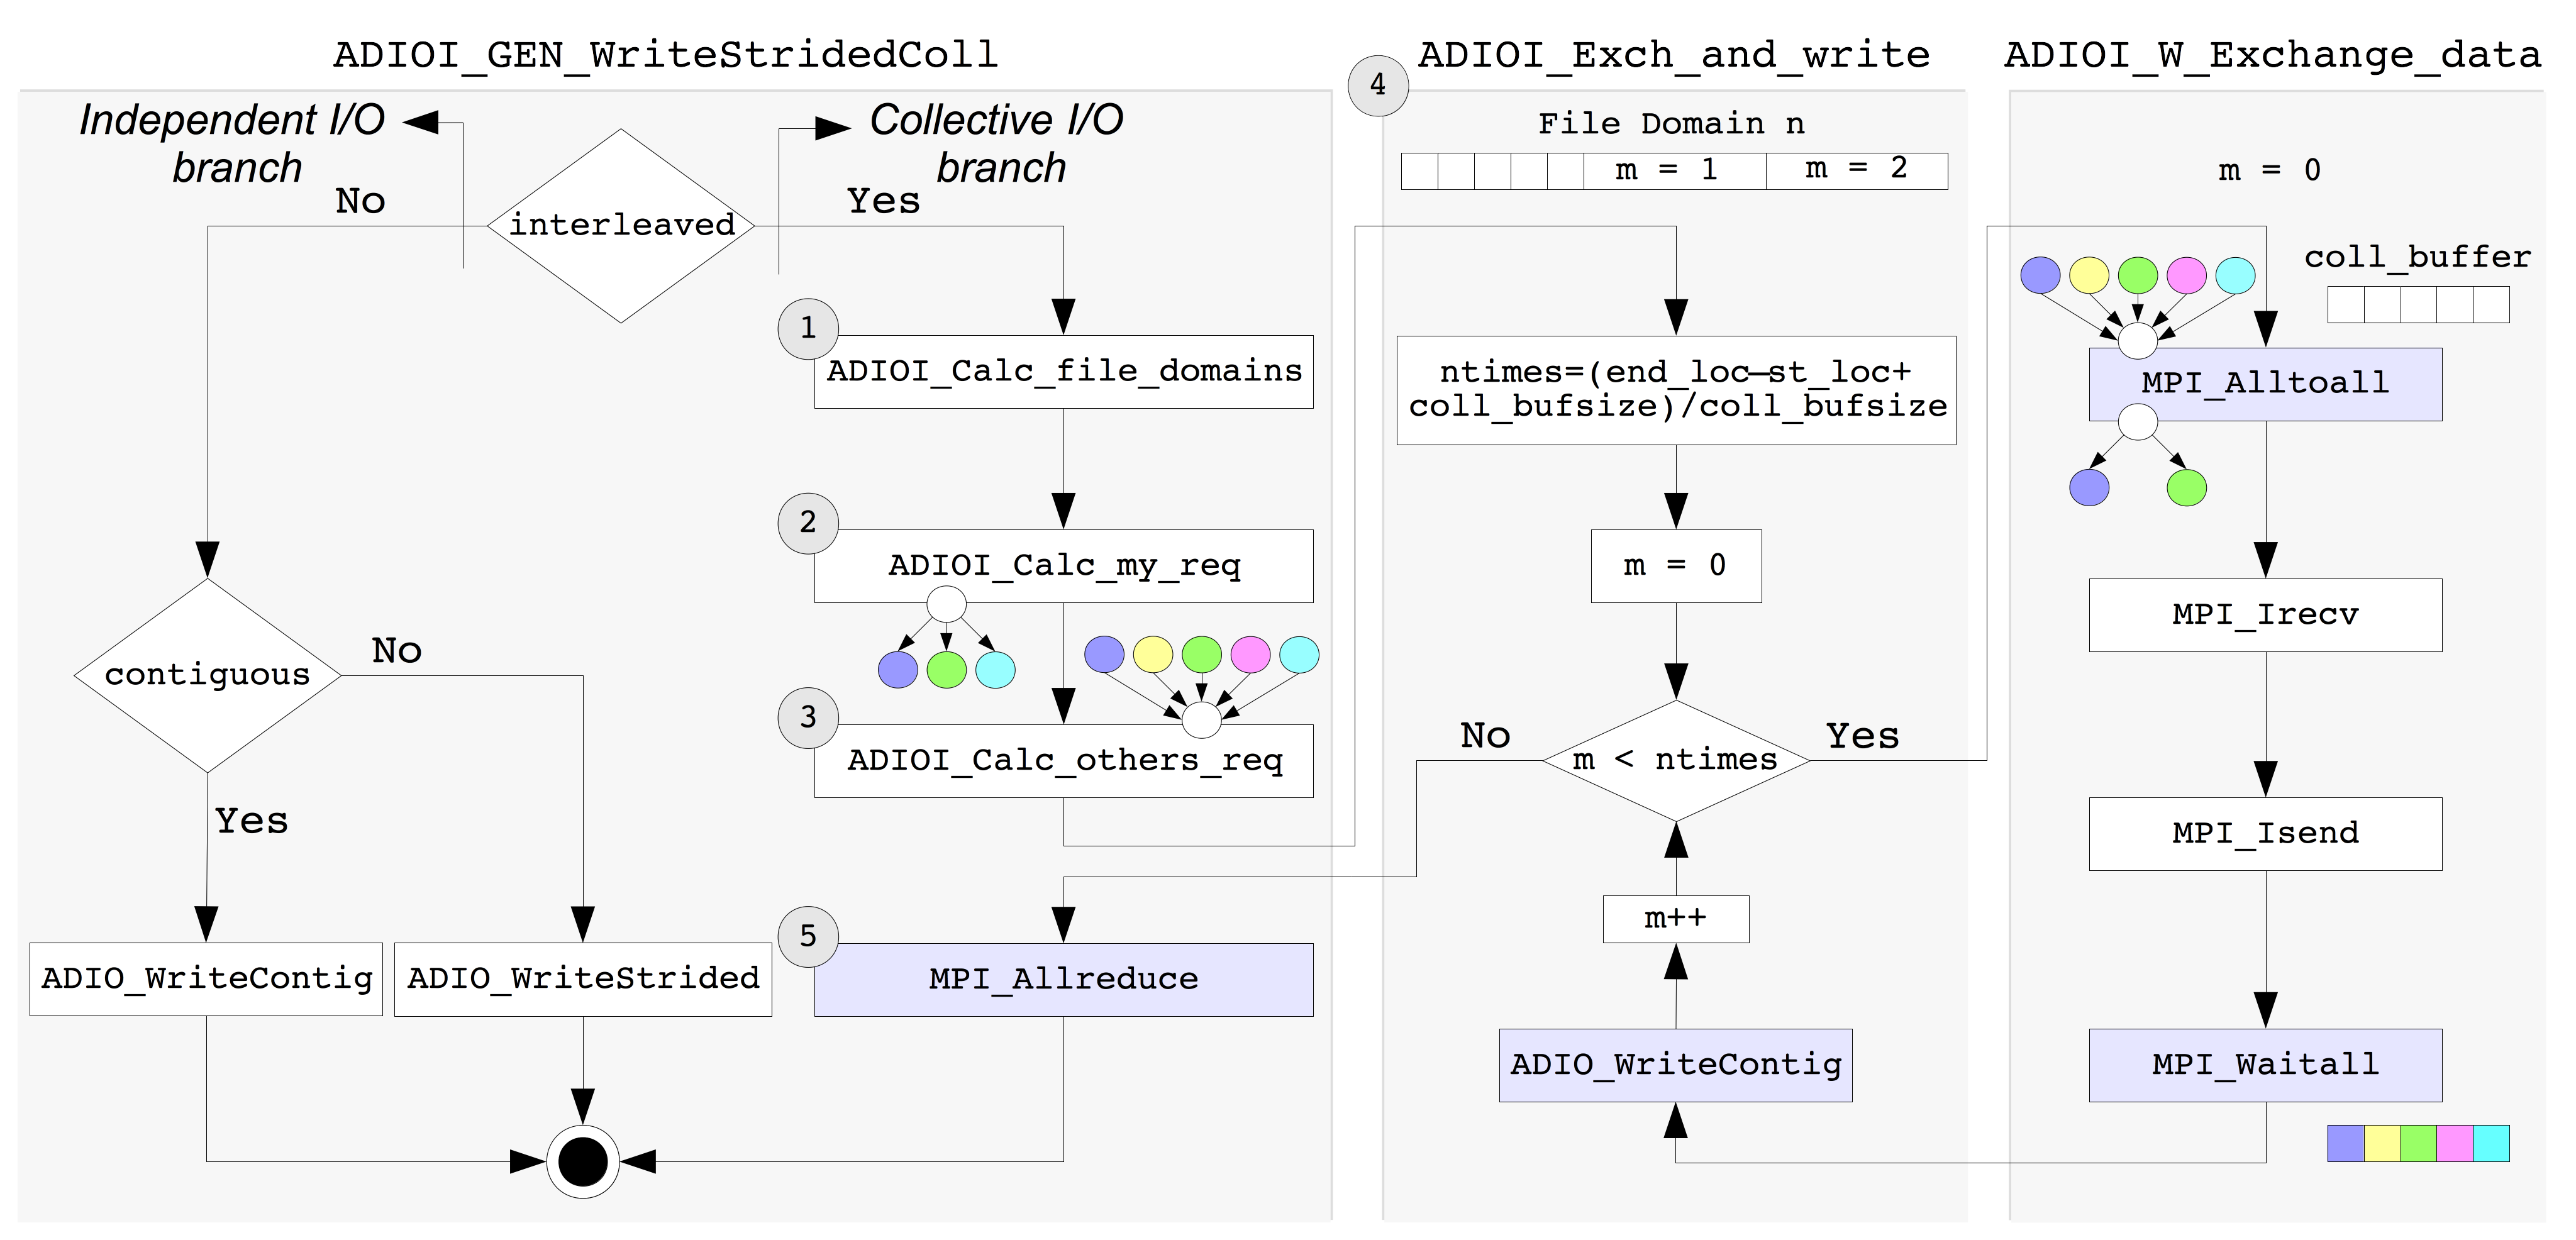
\includegraphics[width=\textwidth]{chapters/chapter3/figures/ext2ph}
  \caption{Collective I/O flow diagram for the write path in aggregators (non-aggregators neither receive nor write any data, just send it to aggregators). \codeword{MPI\_File\_write\_all()} invokes \codeword{ADIOI\_GEN\_WriteStridedColl()}. \codeword{ADIO\_WriteContig} is a macro that is replaced by \codeword{ADIOI\_GEN\_WriteContig()}. Performance critical functions for the collective I/O branch are highlighted in grey.}
  \label{figure: coll_io_impl}
\end{figure}

\begin{enumerate}
\item All processes taking part in the I/O operation exchange access pattern information with each other. The access pattern information is represented by start and end offsets for the accessed region (disregarding holes that may be present). Once file offsets are available, every process works out how big the global accessed region in the file is by taking maximum and minimum among all. The resulting byte range is divided by the number of available aggregators to build the so called `file domains' (contiguous byte ranges accessed independently by every aggregator).
\item Every process works out which file domains (and thus aggregators) its local data belongs to. In doing so, every process knows which aggregators it has to send (receive) data to (from), if any.
\item Every aggregator works out which other processes' requests map to its file domain. Doing so every aggregator knows what processes need to receive (in case of reads) or send (in case of writes) data for that particular file domain.
\item Actual two phase I/O starts. In the case of writes, that we exclusively consider here (the read case is similar), every process sends its data to the right aggregators (data shuffle phase) while these write the data to the parallel file system (data I/O phase). Data is written in blocks of predefined size (collective buffer size). If the size of the collective buffer is smaller than the file domain, the file domain is broken down into multiple sub-domains which are written in different rounds of the ext2ph algorithm. In order to handle multiple rounds of data shuffle and I/O, additional access information is required. This is disseminated by every process (collectively) to aggregators at the beginning of the data shuffle phase.
\item Once all the data has been written, all the processes must synchronise and exchange error codes. This is necessary to guarantee that it is safe to free the memory buffers containing the data.
\end{enumerate}

Figure~\ref{figure: coll_io_impl} shows how the previous steps map to the collective I/O implementation for the write operation. The collective write function (\codeword{MPI\_File\_write\_all()}) in ADIO is implemented through \codeword{ADIOI\_GEN\_WriteStridedColl()}. This is responsible for selecting the most suitable I/O method between those available. For example, independent I/O is selected if the access requests are not interleaved. Nevertheless, users can always enforce collective I/O by setting the appropriate MPI-IO hint. The \codeword{ADIOI\_Exch\_and\_write()} function contains the ext2ph algorithm implementation, including data shuffle and write methods. At the beginning of the data shuffle (\codeword{ADIOI\_W\_Exchange\_data()}) we have the dissemination function (\codeword{MPI\_Alltoall()}) used to exchange information concerning which part of the data has to be sent during a particular round of two phase I/O. 

There are three main contributors to collective I/O performance: (\textbf{a}) global synchronisation cost; (\textbf{b}) communication cost; and (\textbf{c}) write cost. \codeword{MPI\_Allreduce()} and \codeword{MPI\_Alltoall()} account for the global synchronisation cost. When a process reaches them it has to wait for all the other processes to arrive before continuing. \codeword{MPI\_Waitall()} accounts for communication cost since every process first issues all the non-blocking receives (if any) and sends, and afterwards waits for them to complete (refer to the right part of the diagram in Figure~\ref{figure: coll_io_impl}). Finally, \codeword{ADIO\_WriteContig()} accounts for write cost.

\subsubsection{Collective I/O Hints}
\label{subsec: hints}
As already said, collective I/O behaviour can be controlled by users through a dedicated set of MPI-IO hints. Users can control whether collective I/O should be enabled or disabled with \codeword{romio\_cb\_write} and \codeword{romio\_cb\_read}, for write and read operations respectively, how many aggregators should be used during a collective I/O operation with \codeword{cb\_nodes} and how big the collective buffer should be with \codeword{cb\_buffer\_size}. Table~\ref{table: coll_io_hints_table} summarises the hints just described (these are also reported in Table~\ref{table: romio-hints} along with all the other hints).

\begin{table}[!htb]
\centering
\ra{1.5}
\caption{Collective I/O hints in ROMIO.}
\newcolumntype{K}{>{\centering\arraybackslash} m{3cm}}
\newcolumntype{V}{>{\centering\arraybackslash} m{5.5cm}}
\begin{tabular}{KV}
\toprule
\bf \small Hint & \bf \small Description \\
\midrule
\small \codeword{romio\_cb\_write} & \small \codeword{enable} or \codeword{disable} collective writes \\
\small \codeword{romio\_cb\_read} & \small \codeword{enable} or \codeword{disable} collective reads \\
\small \codeword{cb\_buffer\_size} & \small set the collective buffer size [bytes]\\
\small \codeword{cb\_nodes} & \small set the number of aggregator processes\\
\bottomrule
\end{tabular}
\label{table: coll_io_hints_table}
\end{table}

Each of these hints has an effect on collective I/O performance. For example, by increasing the number of aggregators there will be a higher number of nodes writing to the parallel file system and thus a higher chance that one of these will experience variable performance due to load imbalance among available I/O servers, with increasing write time variation and associated global synchronisation cost. Furthermore, by increasing the collective buffer size users can reduce the number of two phase I/O rounds and, consequently, the number of global synchronisation events. Bigger collective buffers will also affect the write cost since more I/O servers will be accessed in parallel potentially increasing the aggregated I/O bandwidth.

Besides the hints described in Table~\ref{table: coll_io_hints_table}, there are other hints that do not directly concern collective I/O but affects its performance. The first is the \codeword{striping\_factor} hint, which defines how many I/O targets will be used to store the file. The second is the \codeword{striping\_unit} hint, which defines how big the data chunks written to each I/O target will be (in bytes). These two hints change the file characteristics in the parallel file system and typically the striping unit also defines the locking granularity for the file in the file system (e.g. Lustre).

%!TEX root = ../../main.tex
\section{The POSIX Advice API}
\label{sec: posix_advice_api}
The Linux kernel allows users to control page cache functionalities through the \texttt{posix\_fadvise()} system call: $$\textit{\textbf{int} posix\_fadvise(\textbf{int} fd, \textbf{off\_t} offset, \textbf{off\_t} len, \textbf{int} advice)}$$ This system call takes four input parameters: a valid file descriptor representing an open file, starting offset and length of the file region the advice will apply to, and finally the type of advice. The implementation provides five different types of advice, that reflect different aspects of caching. 

\begin{table}[!htb]
\centering
\ra{1.5}
\caption{Values for \textit{advice} in the \textit{posix\_fadvise()} system call}
\newcolumntype{K}{>{\centering\arraybackslash} m{4cm}}
\newcolumntype{V}{>{\centering\arraybackslash} m{5cm}}
\begin{tabular}{KV}
\toprule
\bf \small Advice & \bf \small Description \\
\midrule
\small \ttfamily POSIX\_FADV\_SEQUENTIAL & \small file I/O pattern is sequential \\
\small \ttfamily POSIX\_FADV\_RANDOM & \small file I/O pattern is random \\
\small \ttfamily POSIX\_FADV\_NORMAL & \small reset file I/O pattern to normal \\
\small \ttfamily POSIX\_FADV\_WILLNEED & \small file range will be needed \\
\small \ttfamily POSIX\_FADV\_DONTNEED & \small file range won't be needed \\
\small \ttfamily POSIX\_FADV\_NOREUSE & \small file is read once (not implemented) \\
\bottomrule
\end{tabular}
\label{table: advice_table}
\end{table}

The first two advice in Table~\ref{table: advice_table} have an impact on spatial locality of elements of the cache. \texttt{POSIX\_FADV\_SEQUENTIAL} can be used to advise the kernel that a file will be accessed sequentially. As result the kernel will double the maximum read-ahead window size in order to have a greedier read-ahead algorithm. \texttt{POSIX\_FADV\_RANDOM}, on the other hand, can be used when a file is accessed randomly and has the effect of completely disabling read-ahead, therefore only ever reading the requested data. Finally, \texttt{POSIX\_FADV\_NORMAL} can be used to cancel the previous two advice-messages and reset the read-ahead algorithm to its defaults. These three advice types apply to the whole file, the offset and length parameters are ignored for these `modes'.

Two of the remaining three advice types have an impact on the temporal locality of cache elements. \texttt{POSIX\_FADV\_WILLNEED} can be used to advise the kernel that the defined file region will be accessed soon, and therefore the kernel should prefetch the data and make it available in the page cache. \texttt{POSIX\_FADV\_DONTNEED} has the opposite effect, making the kernel release the specified file region from the cache, on the condition that the corresponding pages are clean (dirty pages are not released). Finally, the implementation for \texttt{POSIX\_FADV\_NOREUSE} is not provided in the kernel. %Table~\ref{table: advice_table} summarizes all the advice types just described.

One important aspect of \texttt{posix\_fadvise()} is that it is a synchronous system call. This means that every time an application invokes it, it blocks and returns only after the triggered read-ahead operations have completed. This represents a big limitation especially if we consider \texttt{POSIX\_FADV\_WILLNEED} that may need to prefetch an arbitrarily large chunk of data. In this scenario the application may be idle for a long period of time while the data is being retrieved by the file system.

%!TEX root = ../../main.tex
\section{The GPFS Hints API}
\label{sec: gpfs_hints_api}
Similarly to POSIX advice, GPFS provides users with the ability to control page pool functions through the \texttt{gpfs\_fcntl()} subroutine: $$\textit{\textbf{int} gpfs\_fcntl(\textbf{int} fileDesc, \textbf{void}* fcntlArgP)}$$ The subroutine takes two inputs: the file descriptor of the open file that hints will be applied to, and a pointer to a data structure residing in the application's address space. The indicated data structure contains all the information regarding what hints should be sent to GPFS. Specific hints are described by means of additional data structures that are contained in the main struct. Table~\ref{table: hints_table} summarizes all the available hints data structures and reports the corresponding description for each of them.

\begin{table}[!htb]
\centering
\ra{1.5}
\caption{GPFS hint data structures}
\newcolumntype{K}{>{\centering\arraybackslash} m{4.2cm}}
\newcolumntype{V}{>{\centering\arraybackslash} m{6cm}}
\begin{tabular}{KV}
\toprule
\bf \small Hint data structure & \bf \small Description \\
\midrule
\small \ttfamily gpfsAccessRange\_t & \small defines a file range to be accessed \\
\small \ttfamily gpfsFreeRange\_t & \small defines a file range to be released \\
\small \ttfamily gpfsMultipleAccessRange\_t & \small defines multiple file ranges to be accessed \\
\small \ttfamily gpfsClearFileCache\_t & \small releases all the page pool buffers for a certain file \\
\bottomrule
\end{tabular}
\label{table: hints_table}
\end{table}

Hints are not mandatory and GPFS can decide to accept or ignore them depending on specific conditions. Let us consider the multiple access range hint as an example (\texttt{gpfsMultipleAccessRange\_t} in table~\ref{table: hints_table}). The data structure corresponding to this hint is reported in Listing~\ref{list: mar}. 

\begin{lstlisting}[language=C, caption=Multiple Access Range Hint Data Structure, label={list: mar}]
#define GPFS_MAX_RANGE_COUNT 8

typedef struct
{
    int structLen;
    int structType;
    int accRangeCnt;
    int relRangeCnt;
    gpfsRangeArray_t accRangeArray[GPFS_MAX_RANGE_COUNT];
    gpfsRangeArray_t relRangeArray[GPFS_MAX_RANGE_COUNT];

} gpfsMultipleAccessRange_t;
\end{lstlisting}

\texttt{gpfsMultipleAccessRange\_t} contains two range arrays instead of just one: \texttt{accRangeArray}, used to define \texttt{accRangeCnt} blocks of the file that GPFS has to prefetch, and \texttt{relRangeArray} used to define \texttt{relRangeCnt} blocks of the file previously requested using \texttt{accRangeArray} and that are no longer needed. Unlike posix\_fadvise the user has to manage the list of blocks for which hints have been sent, updating whether they are still needed. Indeed, if the accessed blocks are not released, GPFS will stop accepting new hints once the maximum internal number of prefetch requests has been reached. 

\begin{lstlisting}[language=C, caption=Multiple Access Range Hint Initialisation and Submission, label={list: mar_example}]
void mercury::BlockCache::gpfsAccessReleaseBlock(
    std::vector<mercury::block_t>& access, 
    std::vector<mercury::block_t>& release)
{
  struct
  {
    gpfsFcntlHeader_t hdr;
    gpfsMultipleAccessRange_t marh;
  } accHint;

  accHint.hdr.totalLength = sizeof(accHint);
  accHint.hdr.fcntlVersion = GPFS_FCNTL_CURRENT_VERSION;
  accHint.hdr.fcntlReserved = 0;
  accHint.marh.structLen = sizeof(accHint.marh);
  accHint.marh.structType = GPFS_MULTIPLE_ACCESS_RANGE;
  accHint.marh.accRangeCnt = access.size();
  accHint.marh.relRangeCnt = release.size();

  for (i = 0; i < accHint.marh.accRangeCnt && 
      i < GPFS_MAX_RANGE_COUNT; i++)
  {
    accHint.marh.accRangeArray[i].blockNumber = 
      access[i].blockNumber_;
    accHint.marh.accRangeArray[i].start = 
      access[i].startOffset_;
    accHint.marh.accRangeArray[i].length = 
      access[i].blkLen_;
    accHint.marh.accRangeArray[i].isWrite = 
      access[i].isWrite_;
  }
  for (i = 0; i < accHint.marh.relRangeCnt && 
      i < GPFS_MAX_RANGE_COUNT; i++)
  {
    accHint.marh.relRangeArray[i].blockNumber = 
      release[i].blockNumber_;
    accHint.marh.relRangeArray[i].start = 
      release[i].startOffset_;
    accHint.marh.relRangeArray[i].length = 
      release[i].blkLen_;
    accHint.marh.relRangeArray[i].isWrite = 
      release[i].isWrite_;
  }

  /* issue the hints to gpfs */
  if (gpfs_fcntl(fd_, &accHint))
  {
    std::cerr << "gpfs_fcntl access hint failed for " <<
      fd_ << " errno=" << errno << " errorOffset=" <<
      accHint.hdr.errorOffset << std::endl;
    exit(EXIT_FAILURE);
  }

  /* remove the accessed and released blocks */
  access.erase(access.begin(), 
    access.begin() + accHint.marh.accRangeCnt);
  release.erase(release.begin(), 
    release.begin() + accHint.marh.relRangeCnt);
}
\end{lstlisting}

Listing~\ref{list: mar_example} shows an example for the multiple access range hint initialisation and submission. In the example the \codeword{gpfsAccessReleaseBlock()} function receives two vectors, each containing a number of regions that have to be prefetched (\texttt{access}) and released (\texttt{release}). Every access and release region defines the block number the current request starts from (\texttt{blockNumber\_}), the start offset inside the block (\texttt{startOffset\_}), the length of the block (\texttt{blkLen\_}) and if the request is a read or a write (\texttt{isWrite\_}). For every requested range the implementation fills the \codeword{accRangeArray} and the \codeword{relRangeArray} and finally submits the data structure to \codeword{gpfs\_fcntl()} to be served.


\cleardoublepage
%*******************************************************************************************
% END OF CHAPTERS
%*******************************************************************************************

%*******************************************************************************************
% BIBLIOGRAPHY
%*******************************************************************************************
\cleardoublepage
\addcontentsline{toc}{chapter}{Bibliography}

\bibliographystyle{plain}
\bibliography{bibliography}

%*******************************************************************************************
% LIST OF FIGURES
%*******************************************************************************************
\listoffigures
\cleardoublepage

%*******************************************************************************************
% LIST OF TABLES
%*******************************************************************************************
\listoftables
\cleardoublepage

%*******************************************************************************************
%END BIBLIOGRAFIA
%*******************************************************************************************
\end{document}
%*******************************************************************************************
%*******************************************************************************************
%  END   DOCUMENT 
%*******************************************************************************************
%*******************************************************************************************
